% smrdoc.tex V2.0, 13 May 2010
\documentclass[times]{smrauth}

% Added packages
\usepackage{url}
\usepackage[utf8]{inputenc}
\usepackage{listings}
\usepackage{color}
\usepackage{textcomp}
\usepackage{algorithm}
\usepackage{algpseudocode}
\usepackage{moreverb}
\usepackage[dvips,colorlinks,bookmarksopen,bookmarksnumbered,citecolor=red,urlcolor=red]{hyperref}


\floatname{algorithm}{Pseudo Code}
\def\sectionautorefname{section}
\def\subsectionautorefname{section}
\def\subsubsectionautorefname{section}
\def\figureautorefname{figure}

\definecolor{dark-gray}{rgb}{0.7,0.7,0.7}
\definecolor{gray}{rgb}{0.5,0.5,0.5}
\definecolor{light-gray}{rgb}{0.9,0.9,0.9}

\renewcommand{\algorithmiccomment}[1]{\color{gray}\emph{// #1}\color{black}}

\newcommand{\tvar}[1]{\emph{#1}}
\newcommand{\tdefine}[2]{\textbf{define} \tvar{#1} = #2}
\newcommand{\tquote}[1]{\textquotesingle\textquotesingle#1\textquotesingle\textquotesingle}
\newcommand{\tsingquote}[1]{\textquotesingle#1\textquotesingle}

\newcommand\BibTeX{{\rmfamily B\kern-.05em \textsc{i\kern-.025em b}\kern-.08em
T\kern-.1667em\lower.7ex\hbox{E}\kern-.125emX}}

\def\volumeyear{2010}

\lstdefinestyle{sqlStyle}{
  breaklines=true,                                     % line wrapping on
  language=SQL,
  basicstyle=\tiny,
  keywordstyle=\ttfamily\color{black}\bfseries,
  identifierstyle=\ttfamily\color{black},
  commentstyle=\color{gray},
  stringstyle=\ttfamily\color{dark-gray},
  showstringspaces=false,
  tabsize=2,
  extendedchars=true,
  upquote=true,
  backgroundcolor=\color{light-gray},
  captionpos=b,
  frame=single,
  frameround=tttt,
  fillcolor=\color{light-gray},
  float=h,
  morekeywords={AUTO_INCREMENT, bigint, REFERENCES, CHANGE, NOW, TIMESTAMPDIFF, SECOND}
}

\begin{document}

\runningheads{L. Prévost and O. Liechti}{}

\title{Database Evolution Framework}
%\title{A demonstration of the \LaTeXe\ class file for the
%\itshape{\journalnamelc}\footnotemark[2]}

\author{Laurent Prévost\affil{1,2}, Olivier Liechti\affil{1,2}}
\address{
\affilnum{1}University of Applied Sciences of Western Switzerland, 1400 Yverdon-les-Bains, Switzerland\break
\affilnum{2}Lotaris SA, Galilée 15, 1400 Yverdon-les-Bains, Switzerland}


%\corraddr{Journals Production Department, John Wiley \& Sons, Ltd,
%The Atrium, Southern Gate, Chichester, West Sussex, PO19~8SQ, UK.}

\begin{abstract}

In a service oriented architecture, dealing with the evolution of the underlying database is not a trivial problem. New functional requirements are often associated with modifications of the domain model, hence with modifications of the relational schema. These modifications have to be done in a way that does not impact existing services and applications. They also have to be done in a way that preserves consistency in the data store. Last but not least, they have to be done in a way that has minimal impact on the service availability. In this paper, we propose a framework that supports the development, maintenance and operational activities. The framework consists of processes, tools and best practices. It is the result of our practical experience with a large-scale commercial internet service, which is characterized both by a constant and rapid functional evolution and by strict operational constraints. 

\end{abstract}


\keywords{}

\maketitle

%\footnotetext[2]{Please ensure that you use the most up to date
%class file,
%available from the SMR Home Page at\\
%\href{http://www3.interscience.wiley.com/journal/117946198/grouphome/home.html}{\texttt{http://www3.interscience.wiley.com/journal/117946198/grouphome/home.html}}}

\renewcommand{\thefootnote}{\arabic{footnote}}

\section{Introduction}

Today, the service-oriented architectural style is well understood and is commonly applied to build software systems, across many application domains. IT departments apply it to build corporate information systems, internet start-ups apply it to create on-line services with a global audience. The platforms that support the construction of service-oriented systems, such as Java EE or Microsoft .Net, are now well established. Object-relational mapping frameworks have become very popular and are extensively used. In this context, the design and the implementation of a new information-driven service is a well understood process. A lot of information and documented best practices exist on the topic.

After the initial development phase, however, the situation tends to become much more complex and far less understood. Once the service has been deployed and made available to users, new requirements emerge and drive the evolution of the service. Very often, addressing these requirements requires an extension or a modification of the domain model. New business objects are added, existing business objects are modified, relationships between business objects are altered. These changes materialize in modifications of the underlying database schema and in transformations of the existing data. In an environment, where the same data store is used by a growing collection of services, ensuring that schema and data modifications preserve the behavior of the entire system is not trivial. Furthermore, applying these modifications in a way that fits the operational constraints of the organization is also a challenge. Many software systems are now expected to be available on a continuous basis, with few or no maintenance windows. Upgrading services with minimal downtime is always a challenge, but when data transformations are associated with the upgrade, it becomes a very difficult problem. In addition, the information managed by the evolving system is always a key asset of the organization. Hence, preserving the consistency of this information is of prime importance. Because they may impact on this consistency, the data transformations that are associated with the service evolution have a high associated risk. They have thus to be managed systematically and carefully.

The objective of this article is to propose a framework for dealing with the evolution of data-driven online services. The framework consists of processes, work practices and tools that aim to facilitate the evolution of a service-oriented system, by encompassing the evolution of the underlying information store. The framework is the result from our own experience with the iterative implementation of a global internet service, offered in a ''Software as a Service`` mode. The service is characterized both by a rapid functional evolution and by stringent reliability and availability requirements. 

\subsection{Objectives}

The framework presented in this article is the result of our practical experience with the development and the operation of an internet service with a large and fairly complex underlying database. The pace of development for the service is very fast, with new requirements flowing in constantly. The operational constraints are high, in terms of availability, scalability, performance and security. For these reasons, we are faced with a number of issues when dealing with the evolution of the service. The framework brings answers to some of these issues. As such, it addresses the following key objectives.

\begin{description}
\item[Visibility] Our first objective was to get better visibility on the database evolution. Developers in our team have a shared ownership on the codebase and it is common for all of them to modify the classes that define the domain model. This is true for experienced developers, who are in a good position to assess the impact and the risk associated with the changes. But this is also true for junior developers, who might not always realize that changes in the domain model have an impact on the production database. For this reason, one of the early ideas was to put in mechanisms for tracking and monitoring changes made to the domain model classes. 

\item[Automation and continuous integration] Our second objective was to tightly integrate the database evolution process with the codebase evolution process. In particular, it was to ensure that whenever a developer does a modification in the codebase, he analyzes what modifications are required in the database and he writes the corresponding schema and data transformation scripts. These scripts are first-class citizens and are managed in the version control system. The definition of procedures and guidelines, to be followed by software developers, was seen as an important element to achieve the objective. But it was also foreseen that raising the awareness among the developers and instilling the discipline to write the database transformation scripts was going to be a key element as well.

\item [Correctness and business impact] Our third objective was to ensure the correctness of the database transformation operations. As already mentioned, information in the database is a high-value asset and any inconsistency introduced by a database transformation can have a damaging business impact. It was therefore expected that specific work practices should be defined to minimize the risk associated with the service evolution. Beyond the correctness of the data transformations, the execution of the data transformations can have a significant business impact, because of the service level agreements specified for the system. With many internet services, availability is expected to be continuous and any planned downtime should be as short as possible. For this reason, the time required to execute the transformation scripts needs to be carefully assessed and managed. This is particularly important, because the database underlying an internet service is often very large.

\end{description}


\subsection{Organization}

The framework is a formalization of the work practices, procedures and supporting tools that were introduced in the organization, in order to manage the database evolution process. In this article, our goal is both to describe the framework at a conceptual level and to explain how it has been applied in practice. The remaining sections are organized as follows:

\begin{itemize}
\item In Section 2, we review several approaches to database evolution that have been described in the literature. We look at very practical and pragmatic approaches, but also at more conceptual and theoretical approaches. Our work has been inspired by some of this related work. We consider that our main contributions have been firstly to formalize the developers activities related to database evolution, and secondly to evaluate the proposed practices in a real-word environment.

\item In Section 3, we describe the framework itself. We first look at the different actors involved in the evolution process, such as the developers and the database administrators. We describe their main concerns and needs. We then describe the database evolution process and explain how it relates to the continuous software development process. This leads us to the description of a core activity in the framework, which is the \emph{migration} from one version of the service to another. Based on this, we describe what tasks need to be done on a continuous basis to ensure the success of every migration. We show how simple tooling can make these tasks easier and give visibility on the process. Finally, we describe some of the issues related to testing and validation. We are continuously extending and refining our framework, taking into account the feedback provided by every migration. Testing is clearly an important area that we plan to explore further in the future.

\item In Section 4, we look at the database evolution process from a risk assessment point of view. We provide a list of transformation operations, which are the results of common modifications made on the domain model. We assess both the \emph{risk} and the \emph{complexity} associated with the transformation. We also provide examples to illustrate what we mean by \emph{complexity}.

\item In Section 5, we consider a case study with two objectives. Firstly, we use it to present very practical aspects of the framework. Secondly, we use it to provide evaluation results. The framework, as a set of work practices and supporting tools, is the result of our ongoing work at Lotaris (as such, it is continuously refined and extended). By applying the principles in a real team, on a real service and with real operational constraints, we have been able to identity a set of challenges and pitfalls. We explain how we have been able to address some of them, and how we plan to address the others in the future.

\end{itemize}



Before presenting our Database Evolution Framework, we have a look at what is done elsewhere. We are exploring the tools, the processes and the best practices. Some papers will be described deeper than other in regards of their interests in our approach. After that, we present the framework we have imagined based on our readings and particularly our experience in database evolution management. We want to present how we have used our framework in a real case and for that we will offer you a study case. Finally, we go through what is missing in our framework and what we want to do in the future to improve our methodology and our tools.

\section{Related Works}

% http://se-pubs.dbs.uni-leipzig.de/

During our investigation, we found different approaches to the problematic, some of them bring some solution with tools and the other ones are only best practices and processes. None of them have solved our requirements entirely even if we found a lot of ideas that we have used intuitively before reading the papers or that we have integrate since we discovered them. We will start to describe the process oriented papers and after that the tools.

\subsection{Database refactoring}

In software engineering, the concept of code refactoring is well known and has become a standard practice. According to Fowler \cite{fowler_evolutionary}, refactoring is defined as \emph{``the process of changing a software system in such a way that it does not alter the external behavior of the code yet improves its internal structure''}. Code refactoring is an important practice in agile software development. It encourages programmers to start with a system design that is as simple as possible, and to add complexity iteratively in response to new requirements. Code refactoring is closely related to unit testing, because having a collection of automated tests makes the refactoring process much less risky (running the tests is a way to verify that the external behavior has not been affected by the refactoring).

In \cite{ambler_process_2011}, Ambler has introduced the related notion of \emph{``database refactoring''}, with the following definition: \begin{quote}\textit{A database refactoring is a small change to your database schema which improves its design without changing its semantics (e.g. you don't add anything nor do you break anything).  The process of database refactoring is the evolutionary improvement of your database schema so as to improve your ability to support the new needs of your customers, support evolutionary software development, and to fix existing legacy database design problems.}\end{quote}

Ambler explains that a database refactoring can be more or less difficult, depending on the number of applications built on top of the database. When a single application is built on top of the database, the impact can be relatively easy to assess. When several applications are built on top of the database, the impact analysis is much more complex. This is particularly true if the applications are managed by different organizations. Of course, whether or not the applications built on top of the database are covered by unit tests makes a huge difference when it comes to measure the impact of a refactoring.

Ambler describes database refactoring as a three-step process. The process starts in the development sandbox, is implemented in the integration sandbox and finally installed into production. While initiating the work in the development sandbox, the developer should go through a sequence of well-defined steps. After assessing the need to perform the refactoring, developers should implement unit tests, write schema modification and data transformation scripts, run tests and make sure that their scripts are under version control. Ambler also refers to an interesting idea, introduced by Sadalage and Schuh \cite{sadalage_agile_database}: the notion of a \emph{deprecation} (or \emph{transition}) \emph{period}. The idea is that a change in the database schema cannot be taken into account immediately by all applications. During the transition period, all applications should still work, some of them using the new schema and others using the old one. Mechanisms, such as triggers, can be used to keep the data consistent under such circumstances.

Our framework has several elements in common with the process described by Ambler. Firstly, it also describes concrete procedures, with well-defined steps, that have to be followed by developers (i.e. it is quite prescriptive). Secondly, it has been developed in an agile development organization. New requirements are frequent, and so are the are the needs to perform database transformations.

\subsection{Migration process}

David Katzoff \cite{katzoff_how_2011} offers a solution to test the data migrations. First of all, he demonstrates that the sampling approach is not suitable for all the cases. With this approach, not all the data are verified that will not ensure all the data keep their integrity. He proposes to do Pre-Migration testing that brings a couple of actions before any migration procedure, followed by a Formal Design Review that describe the source and target systems, quantity of migrations (data, queries, ...), resources required, time required and so on. After that, Post-Migration Testing are done to detect any defect. These tests are done on a sandbox environment that is specific for data migration and allow testing. Finally, the User Acceptance Testing could be done to detect any other defects that could not be found automatically. Once these tests are done, the Production Migration is ready to be done. Finally, David Katzoff offers ten recommendations to handle data migrations from process point of view.

This methodology is specially appreciated when your software development process is planned on a relative long period (more than two weeks). In our case, we use the SCRUM\cite{schwaber_agile_2002}, \cite{scrum} methodology to manage our development. In this methodology, we organize our develiveries in terms of sprints of two weeks duration. In other terms, it means that we could potentially have migrations every two weeks. We cannot manage such a process as propose by David Katzoff due to the people implied in the process and the time potentially consumed. We need to keep as most as possible the agility to add new features with data migration and keep confidence in the application and migrations. In this situation, we need to find a lightweight process to reach a balance between high modifications of data and stability of the applications. 

\subsection{MeDEA}

Metamodel-based Database Evolution Architecture (MeDEA)\cite{Dominguez2008419} offers a generic evolution architecture to maintain the traceability between the different elements involved in database development process. This method is generic because it does not use a specific modeling technique as an input. In the whole system, a translation component between conceptual schemas and logical schemas is used. This is the principal contribution of this approach. The translation element does the conversion between the conceptual and logical schemas with avoiding to start from scratch each conversion. The article concludes with the fact that the system is not designed for huge database with too many data. In this case, the performance and duration during a migration could be really awful.

This methodology brings is specially interesting for the fact that the modifications are planned with a metamodel. They are kept to trace each change in the database. It is designed in a way that any modeling language could be use to prepare the evolution. In our situation, such a system, is not totally appreciated. Some our refactoring implies some unplanned data model modification with an impact on the database schema. This situation required some reverse engineering approach to prepare the migration statements. MeDEA does not offer such a way to track these kind of modifications. One thing that we believe in is the traceability of the data migrations. For that, we want a system with the capability to track the modification to apply and the modification applied. For that, we need a structured approach that could be inspired by systems like MeDEA.

\subsection{DB-MAIN}

DB-MAIN\cite{Hick2006534} approach as the same kind of approach as MeDEA. The approach is centered on the evolution process and tries to address the problems of automatization of the database modifications. The article presents where the modification come from. The modifications come from a specification point of view. The whole solution analyze the way to track and apply the modification on the database and also on the application. One question asked is how to update an application after the database is updated to match the new specifications. One another interesting aspect this paper is the way to manage the modification tracking done by the migration. The history mechanism allows undoing the migrations. Idea is to write the reverse statement (includes all details required for that) that allows coming from a migrated version to an earlier version. There are also some recommendations like when a primary reference is introduced against existent data, the data present must be checked to be safe for the migration. It means that the foreign keys must satisfy the unique constraint check. The authors do the statement that the migrations for renaming, adding relations, attributes, entities or updating a cardinality are more frequent than conceptual refactoring. It means that the impact of such a modification has a less impact than the others. The paper gives the impact of database modification on the programs. For example, adding an attribute is quite transparent for an application.

One more time, the approach of this article comes from the conceptualization of the data store to the application. We do not want to go through this kind of process. Our applications run the process of database modeling through a data binding done by the frameworks we use. In this situation, we cannot apply directly the recommendations, processes and tools describe in this paper but we can study some aspects and use some of them. For example, the way that the history is used with the possibility to rollback any modifications done in a migration is really grateful. The traceability is the key concept to keep an ease of the data migration process. We try to address this at the beginning when the application is modified to the migration executed when the application is deployed. We have also defined the categorizes and risk levels for data migration types. As we have seen for now is that we have a lot of small migrations as the article describes and small amount of major migrations that could have a major impact during the migration execution.

\subsection{PRISM}

The PRISM \cite{curino_prism_2011} tool provides a language to define the migration changes. This language is called SMO\cite{smo} is a language that is not so far from SQL language. You can write the same kind of commands with additional ones. For example, you can write a command to split a table into two tables with \textit{DECOMPOSE TABLE objectcache INTO ob1(keyname, value), ob2(keyname, exptime);}. The figure~\ref{smoLanguage} shows the different commands and translation to relational language. The process used by the tool is defining the SMO queries to update the database schema, viewing the reverse queries (built on the base of forward queries), validating the queries (migration validation) and finally, running the migration (observing the queries).

\begin{figure}[h]
        \centering
        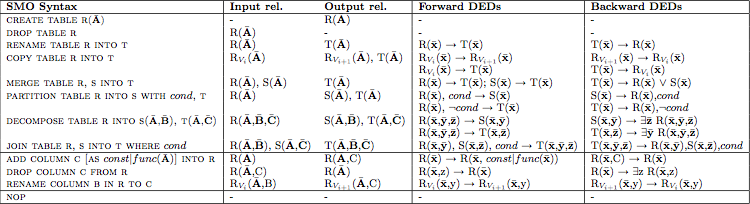
\includegraphics[scale=0.53]{images/Smo-to-ded.png}
        \caption{SMO Language for PRISM \cite{curino_prism_2011}}
        \label{smoLanguage}
\end{figure}

With PRISM, the changes to do must be well known before using the tool. In our case, we use an ORM that masquerade the changes and force us to find a way to detect the changes and which are they. In such a situation, it begins to be more difficult to use a tool to write the changes and one another to detect the changes. In this situation, we cannot use directly such a tool to manage our data migration.

\subsection{DBDeploy}

DBDeploy\cite{ashley_taking_2011} is a tool that provide a way to manage database migrations. The tools offer a way to check a database, retrieve the actual state and build the migration script ready to be run on test environment or production environment. The tool retrieve the actual state of a database directly from the database through a dedicated table that triggers the database evolutions. From there, it has the possibility to create the migration script from the current state to the state wanted by the developer modifications. The author, Nick Ashley, of the tool, describes best practices based partially on the "Database Refactoring" from Scott W. Ambler and also on what Martin Fowler advocates. In summary, it is recommended to work is small unit of change, committing frequently will avoid "check-in Friday" syndrome. Ashley says: "The use of a Continuous IntegrationI\cite{fowler_continuous_integration} tool is core to this method of database refactoring. Building functionality by small steps and rigorously building, deploying and testing the output at every step helps to raise bugs and other integration issues early and as so provide more time for them to be fixed in a more controllable manner." The white paper is based on ant for the usage of the tool but it exists also a Maven\cite{maven} plugin that the documentation could be found on the source code repository\cite{dbdeploy_source}.

One interesting fact in the approach of DBDeploy is the way to store the state of migration script ran into a certain database. The tool has its own table to monitor the database changelog. With this table, it becomes possible to follow the lifecycle of the database. It is possible to store the last migration script ran and the previous ones. Actually, we do not have such a method but it is something that we want to improve. We need a mechanism to monitor which scripts are run and where. Another interesting point, that we actually apply, is the way to manage the migration scripts. For DBDeploy approach, each change to the database \emph{must} have its own atomic script. It means that for each change done in the code must be reflected by a migration even if the change occurs in a short period. As Ashley said, the main point is organized around the CI tools. For us, we also have the same spirit about this kind of tools. We move towards a solution of a nightly build and testing for the specific field of database evolution in addition of our other testing processes.

As DBDeploy looks sexy, it does not address all the needs we are looking for. Actually, we do not need a tool to handle the construction of a final migration script, we already have one home made tool to do that. We need to add a way to know the current state of a specific database and to which state we want to go. Another tool we need is a tool to compare two database and see the delta between them in the context of continuous integration. 

\subsection{MoDEF}

MoDEF\cite{Terwilliger:2010:WDU:1807167.1807316} is an additional built in tool for the IDE\cite{ide} VisualStudio. It brings the capability to automatically writing the migration scripts to evolve a data store when a code change is detected (saved) on the disk in the context of data mapping framework. The tools offers automatism to prepare statements to migrate a database and in this situation, offers a bridge between database administrators and developers. They could discuss on a common base. The tool store the scripts when the code is saved on the hard disk under a log format. The developer can at any time generating the whole script, creation until latest modification, or upgrade a point in the code to the latest modification. The generated script contains comments relative to the updates done in the code that allows following the modifications.

This tool is really promising but only available for Visual Studio and for a specific data mapping framework. It is difficult to adapt it directly to other technologies but this is not the most blocking point. The tool and approach focuses the mapping changes or entity changes in general but the modifications of the data inside the data store is not handled and you could miss some changes that requires a data modification when the application is deployed. One example of this kind of non-monitoring changes could be when you store XML\cite{xml} in your database (the reason will not be discussed there) and you want to change the format of your XML stored in the database. Your schema remains exactly the same after your refactoring of the XML format but your application would not work anymore if you do not apply some data transformation to reflect your XML format change. MoDEF have no way to handle this kind of changes.

One interesting thing in this paper is the way that the modifications are viewed in terms of migration scripts. The atomicity principle for the modification scripts are applied. It means that for each code modification, a log entry is written (only if the code is saved) and a scripts could be generated for the modification. If the modification is reverted later with a new update of the code, another log entry is written for this modification. So another script could be generated to cancelled the previous one. In terms of semantic, each action on the code is logged and a scripts could be applied. In terms of application behavior and migration scripts, some changes could have no effect due to a counter-part script that cancel the previous one.




\section{Towards a Database Evolution Framework}
	\label{sec:def}

% Introduce development lifecycle and show that happens multiple time

Our framework approach is based on some key concepts and some hypothesis. First of them is that the solution developed and managed lied on 

As we have read, usually, Database administrator do not like to change any database schema due to the risk implied by the changes. One minor change at a point of schema could have major repercussions to the whole system you have. In our case, we have only one application per database. This is the ideal case that any DBA dream about it. When you change your code, you can change your database relatively easily due to the fact there is only this application that use the database. You do not impact any other application. You could have one or two exception when you have some reporting application that directly interrogate your database.

With our approach, we want to cover a relative basic approach. We suppose that only one application is concerned by a migration process with no exception (other external data extracting tools). On this base, we are able to build a framework with different identified people, process rules and tools that all together bring a way to handle as best as possible the migration whole process. We also based our processes and tools on the fact that the application use an ORM\cite{orm} that brings high development capabilities but a loss in control in your database access. With the persistence layer that the ORM brings, you have not necessarily the control of the underlying relational data model but you, normally, do not have to write any SQL\cite{sql} in your application. We do this hypothesis that we do not use any native SQL language inside the application. With these differents hypothesis, we do not realize that any change in our data model will greatly implies an impact on our database schema or data.

Let's start with a discussion about the people involved in the process of data migration. We are interested by identifying the role of people in such a way to know what they do in the process and/or what their impacts on the data evolution. We will discuss also about when they step in the lifecycle. When we have an overview of these roles, we could introduce the processes used and who manage them. Finally, to help in the application of the process, we need tools. Some of them are written to suit the processes we offer.

\subsection{People}
	\label{sec:def:people}

We have identified different kind of people that are implied in the whole process of the data migration.

\subsubsection{Customer\\}

The most important people are the customers. Without them, we do not have any business. This is an evidence. They ask for new features, they ask for improvements, they ask for corrections. They are at the center of any evolution triggered by the market needs. When they ask such of modifications, they have no idea of the technical impacts and they do not want especially to be involved with this kind of things. They just want that our product reach their requirements.

\subsubsection{Product owner\\}

The product owner is in charge to manage the evolution of the product. He has a good knowledge of the market and try to anticipate the market needs. He wants that the product evolves to get new customers but also to satisfy current customers. He tries to balance the current features with the new features to introduce to match new requirements from old and new customers. In this position, he has a great interaction with developers due to the fact he basically gives the tasks to developers.

\subsubsection{Project manager\\}

When you offered an application as a service, you have sometimes to integrate partners. These integrations are, in general, managed as projects. We could see this organization as a transverse one. In facts, the project has an impact on the application. The project manager has the same kind of power than a product manager. He tries to balance the requirements of customers and partners to conserve the coherence of the application. He also gives tasks to developers that imply sometimes database evolution. He has a great implication with the product owner.

\subsubsection{Developer\\}
	\label{sec:def:developer}

A developer is the person that have the most impact in terms of technical aspects. He introduces the changes inside the application source code that have the impact on the database. For this reason, this is also the person that is the best placed to know exactly which kind of modification he did and how to handle it. For these reasons, the developer has an important task when he did a modification that impact the database. He has to write migration scripts relating to his modification. He must test them to ensure that the scripts are runnable.

\subsubsection{Migration manager\\}

The migration manager has the role of coordination to follow the migration scripts writing. He tries to know all about the application, to know any change in the data model of the application. He does a first migration scripts review in terms of concern separation. He needs to separate contextual modifications from technical ones. He keeps the scripts organization as cleaner as possible. Finally, he tries to catch missing scripts or erroneous ones. His role is more in coordination than technical. He could also have the role of developer in writing scripts. He must be an example by following the rules and teaches them to others.

\subsubsection{Database administrator\\}

Database administrators manage the databases for performances, integrity, maintenance operations. But he has also an important role of migration code review. He must be able to get the migrations scripts written by developers to run them. He must be able to validate that the scripts technically run against a database that must be upgraded. He is also there to give feedbacks to developers when the migration scripts must be improved due to lack of performances. 

\subsubsection{System administrator\\}

The system administrator, in addition of maintaining the system running, has in charge the application migration. With the help of DB Administrators, he has to run the migration scripts during the application migration. He must provide sandbox environments for migration testing in the most nearest production way as possible. The application migration must be run in the nearest real conditions. He ensures the execution of the migration process. He will also do the migration on the real environments when the sandbox ones will be validated by Quality Assurance team.

\subsubsection{Quality assurance agent\\}

To ensure the migration keep the application correct and functional from end user point of view, we need people able to run manual and automatic tests agains the migrated application. The quality assurance agent has the responsibility to test the application after a migration and validates that technical all is correct but also from business point of view. He needs to validate that the application reacts as the customers asked and also ensure that all data keep integrity, no data loss, no side effects on the data. He will give the ok/nok for the production application migration. The quality assurance agent could be internal people or external people. Customers could provide their quality assurance agents to keep a regard on the migration process.

\subsubsection{End user\\}

The end user is the person that use the application offered by our customers. We do not address directly the end user but we have a big incidence for their user experience. With their feedbacks to our customers, we will have corrections and/or improvements. At all, the migration process starts and ends with the end users inputs (directs or indirects). Any process has its weakness. 

\subsubsection{Summary}

We can summarize the previous roles as stories to help us in the definition of the process part.

\begin{itemize}
\renewcommand{\labelitemi}{$\bullet$}
\item As a customer, I want to be sure that a new version of the system do not corrupt actual data
\item As a customer, I want to be sure new features are implemented as I need and will use data correctly
\item As a product owner, I want the insurance that the system keep the correctness of data after migration
\item As a product owner, I want to be sure that the requirements based on the data already present in the application
\item As a project manager, I have the same concerns as a product owner
\item As a project manager, I want to have the insurance that our data are equivalent to partners data when we need reconciliation
\item As a developer, I want to develop with ease and flexibility without worrying to much about the data migration.
\item As a developer, I need a way to write migration scripts quite easily with well defined procedures
\item As a migration manager, I want to keep a trace of the data model modification or any database relating updates
\item As a migration manager, I need tools to help me to track changes and to build final migration scripts
\item As a migration manager, I need to have procedure to follow migration scripts writing progress
\item As a database administrator, I want to be sure that I can dispose migration scripts when it is necessary
\item As a database administrator, I need to run the migration scripts at any time to do testing and ask for improvements
\item As a system administrator, I want to be sure that the application migration could be done with the minimal risk of migration rollback
\item As a system administrator, I will provide sandbox environments to test migration scripts and application migration
\item As a system administrator, I run the application migration on the different environments (with/without help of DB Admistrator)
\item As a QA agent, I want to have the possibility to test the application after migration in a sandbox environment
\item As a QA agent, I need to automatize the tests to have a more complete testing process
\item As a QA agent, I will give the go or no go to a production application migration (with the approval of customers)
\item As an end user, I want to have the best user experience without worrying about the technologies used to offer me the services I used
\item As an end user, I do not want to encounter major issues due to application updates
\end{itemize}

\subsection{Process}
	\label{sec:def:process}

Our framework relies on processes and tools that we combine to manage the different database evolution. For the next paragraphs, we assume that a code versioning system is used to manage the code. This system is able to use a plugin system to add some actions at different point in the versioning process such code is manipulated in the versioning system. The framework is agnostic for the choice of such a system or which database engine used by the application.

The process to manage the migration process requires several steps. First of all, it is necessary to monitor the code modification to detect any change that could imply a database evolution. After that, we need to ensure that the migration scripts are written and correct. Then, we need to run the migration script on a sandbox environment to ensure the correctness on a database that contains data in production way. Finally, when all is fine, we could run the migration on the production environment. The Fig. \ref{fig:migrationProcess} summarize the migration process.

\begin{figure}[h]
        \centering
        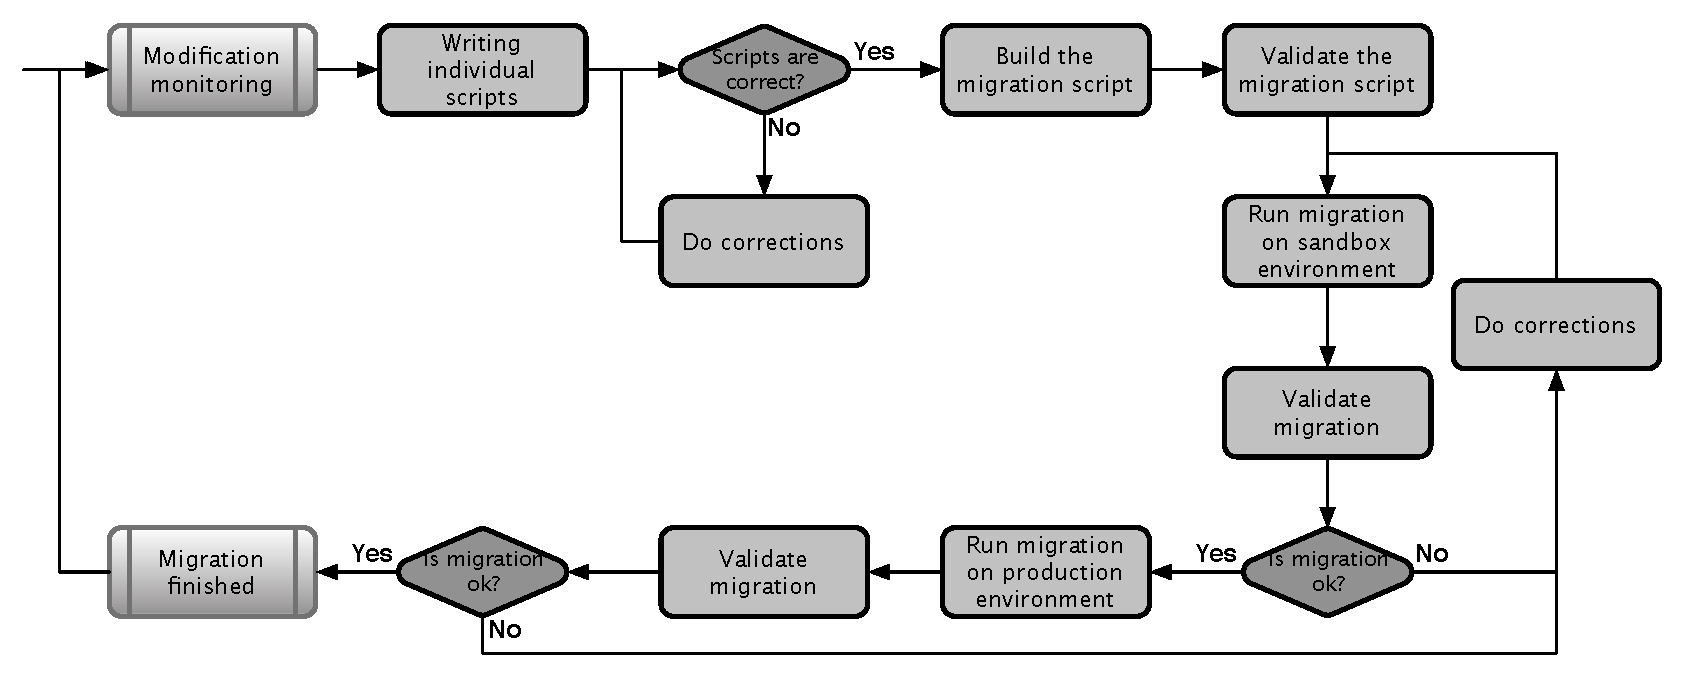
\includegraphics[scale=0.50]{images/MigrationProcess.pdf}
        \caption{Migration process}
        \label{fig:migrationProcess}
\end{figure}

One part of the whole process of data migration is to track the data model transformations. As we know, we have defined different kind of data transformation. We have structural refactoring that implies schema transformation (adding a column, adding a table, removing column, data type modification and so on). We have data migration that imply to work on the data present in the database. In this case, we can divide in two groups, the data that are generic (called infrastructural data) and data that are used in the application deployment (called contextual data). Depending on which transformations, the migration process is slightly different and more work is required to ensure correct evolution. For further details, refer to \autoref{sec:risks}.

When the modification are tracked, it is important to check the migration writing process and to enforce some rule for the migration scripts writing. On the Fig. \ref{fig:migDetProc}, we suggest a process to monitor and ensure that the migration scripts are written and are correct. Basically, the first step for this process is the monitoring of the data model modifications. When such a modification is caught, a short analysis is done to ensure if a script is required for the modification detected or not. If a modification is required, another process is required to ensure that the migration is correct and follows the migration writing rules. Finally, all this monitoring is kept in a file to track at any time the state of the migration scripts. We offer a format that could be used for that in Fig. \ref{fig:migTemplate}.

At this point, the migration monitoring process will be done regularly to avoid any delays in the migration writing process to ensure that at any time, the migration scripts to deploy the applications could be built from the migrations script parts.

\subsubsection{Tracking model modification\\}

As we just discussed previously, one important part of our approach is the data model monitoring to track any modification. This part use actively on the versioning tool in place. In general, these kind of tools allows to add sort of plugins to do extra work after or before any piece of code is injected into the versioning repository. These functionnalities offers a great way to automate some controls. Some scripts can verify if any piece of code could be eligible for a migration scripts. With basic checks, emails could be sent to a mailing list for a further analysis. Some updates could simply comments in the code that are not a modification that requires a migration script.

\begin{figure}[h]
        \centering
        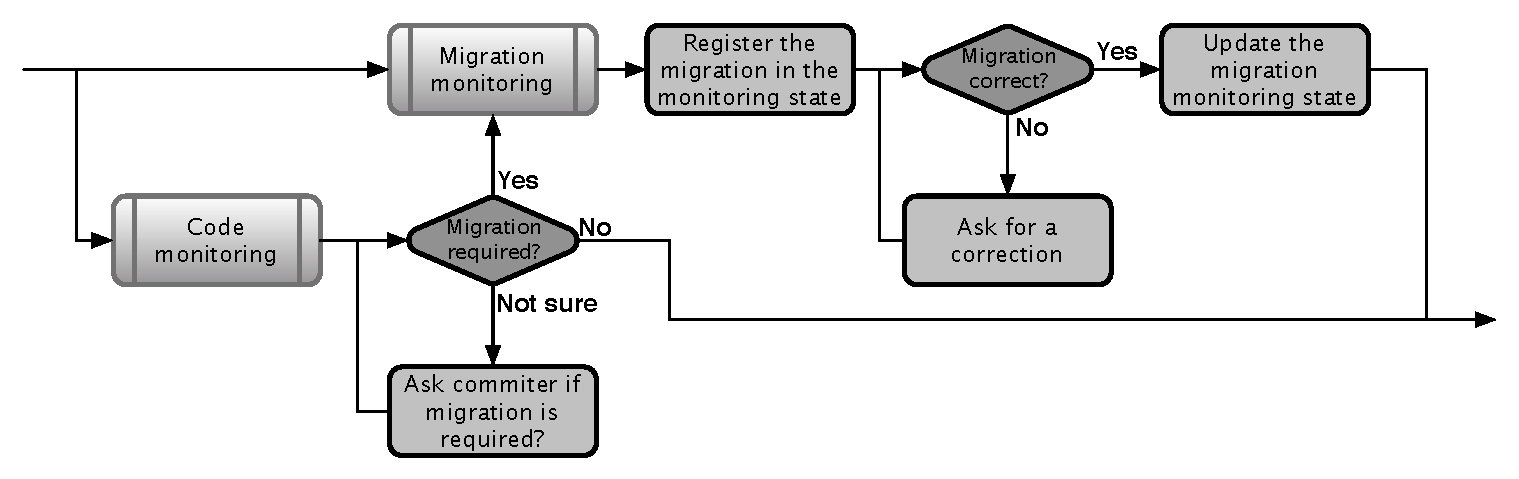
\includegraphics[scale=0.55]{images/MigrationDetetcionProcess.pdf}
        \caption{Migration monitoring process}
        \label{fig:migDetProc}
\end{figure}

When a modification is eligible for a migration script, the migration tracking file must be updated for the revision that contains the modification. The first two columns could be filled with the migration number (basically an incremental number) in the current migration process and the migration name. The commiter column must be filled too.

At this stage, the migration monitoring could start. Each developer that produces a modification that requires a migration needs to write the corresponding migration script. For that, the developers relays to the migration script writing rules described a little bit later in this paper. In the same way that the code modification are monitored, we could do the same for the migration scripts. The first reason is to know that the migration script file is created, when it is created and by which. The second reason allows checking the migration script regularly. This is important to check the correctness of the scripts and ask quickly for modifications if required. A third reason is to check that a script is not modified frequently and for the bad reasons. A migration script must be immutable. It means that we do not want any modifications of scripts expect for corrections. For this step, the columns "Present" and "Correct" are used to know the state of the migration script. The "Remarks" column is a quick help to keep the reason why a script is correct for example. The "Added in" column is filled with the revision identifier when the migration script was commited to the versioning repository.

We also use a "Releated to" column to track the contextual migration in regards of the modifications done in the code. We want to keep the context of the migration and for that we need to know for which revision identifiers the migration is relevant. We will discuss in depth this last part and the naming rules in the section \autoref{sec:rules}.

\begin{figure}[h]
        \centering
        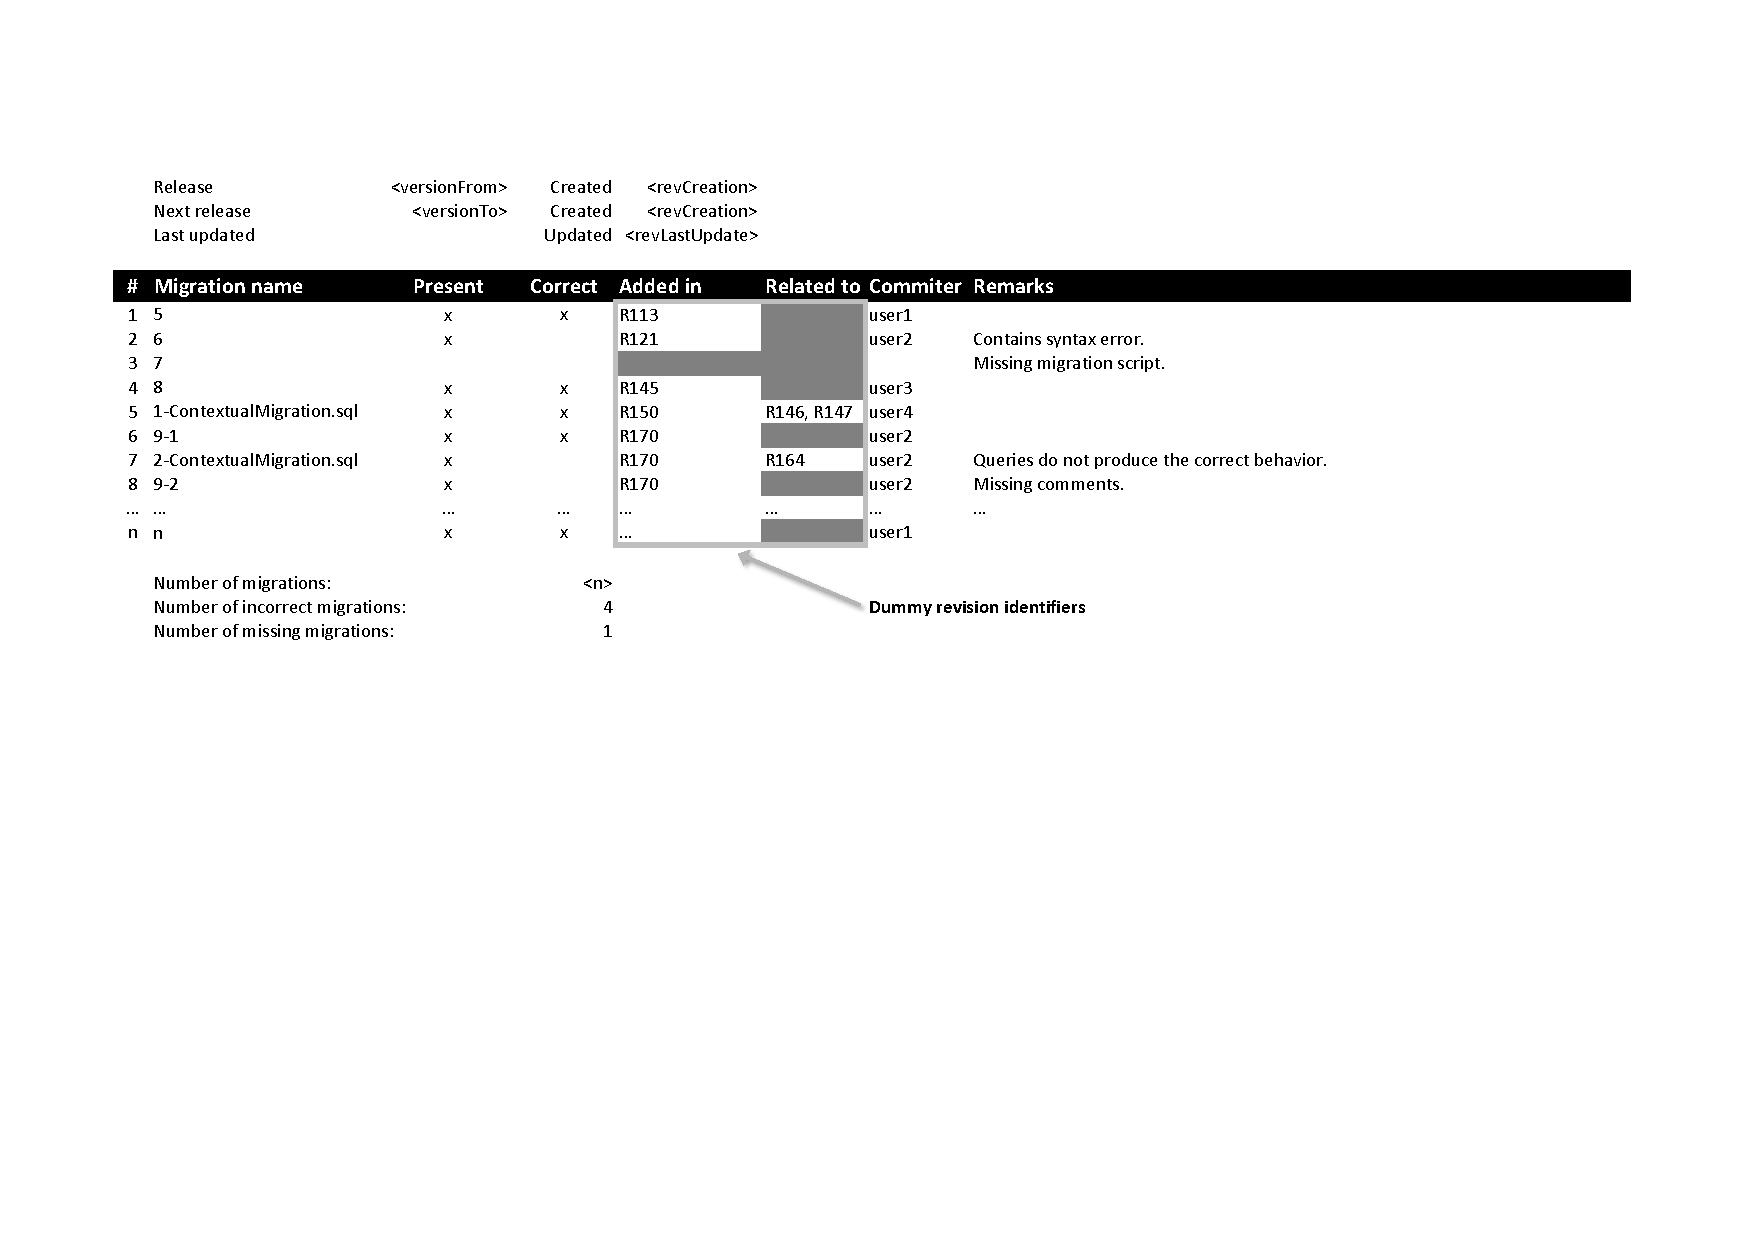
\includegraphics[scale=0.55]{images/MigrationMonitoringTemplate.pdf}
        \caption{Migration monitoring template}
        \label{fig:migTemplate}
\end{figure}

\subsubsection{Migration script writing rules\\}
	\label{sec:rules}

To write a migration script, we need to follow some rules for coherence, easiness and not the least important aspect, to match the format that the migration builder tool use to build the final migration script from the different migration script parts. We will go across the process that define how to write a script, how to name it and such of things. The figure \ref{fig:genMigScriptSchema} will show the whole process to write a script with references to other figures shown after. The figures \ref{fig:genMigScriptSchema-1}, \ref{fig:genMigScriptSchema-2}, \ref{fig:genMigScriptSchema-3} and \ref{fig:genMigScriptSchema-4} will show parts involved in figure \ref{fig:genMigScriptSchema}.

\begin{figure}[h]
        \centering
        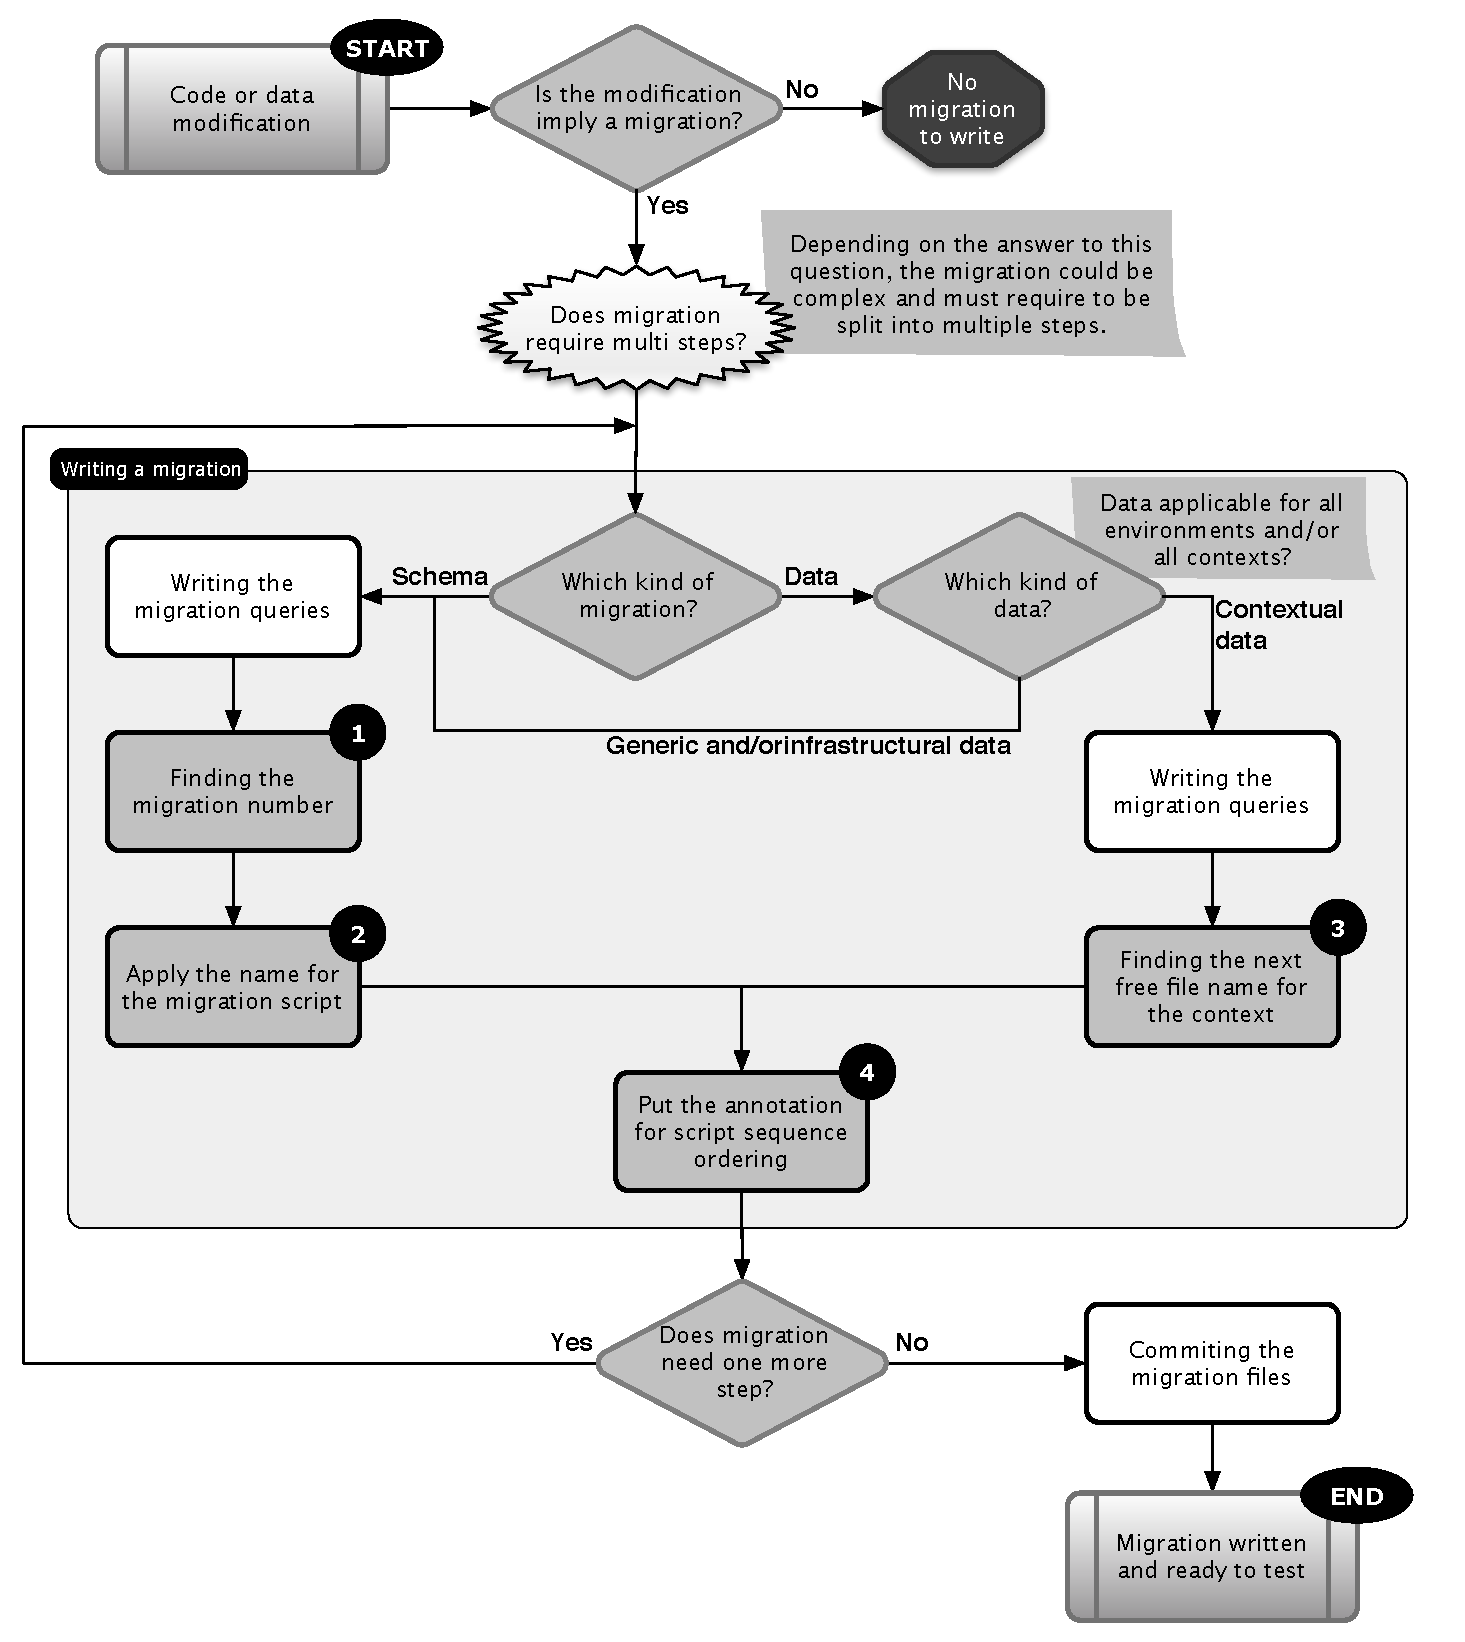
\includegraphics[scale=0.60]{images/mig-schema-gen-main.pdf}
        \caption{How to write a migration script schema}
        \label{fig:genMigScriptSchema}
\end{figure}

As we already discussed, we track the model modification through the help of some script and tools, but the developer who wrote the model modification has the responsibility to provide the corresponding migration script on his own (with the help of his colleagues if necessary). To help him in this task, some rules are in place to know where to put the queries and how to organize the migration. When a script is written, the developer must ask himself some questions to know how to organize his migration script. For example, the first question to ask is if a migration must be split or not?

Why a script could required more than one part? The reason is quite simple. When you manage multiple environments with the same application deployed with their own database (same schema across the different deployments), the data stored are not the same. They could be updated differently from environment to environment. Contextual requirements must be took into account. In this case, when the queries must manipulate the data in a contextual way, splitting migration script into parts is required. Sometimes, this question is not so easy to answer when the developer starts to write his queries. Our writing rules cover this case.

Before starting the script writing, the developer must answer one more question. Which kind of migration is it? Is it schema migration only? Is it migration and data? Is it data only? When there are data migration, the developer must also answer the question about the context of the data. Is the data generic/infrastructural or data are contextual to an environment? Based on the answers given by the developer, the process to write the migration script is slightly different.

Let's continue with an example to go deeper in the migration writing rules. Read the class diagrams on Fig. \ref{fig:classDiagSample} that shows before and after a code modification with impact on the database schema and data. In the "before" modification, we see a simple class that contains a price and a currency in "hardcoded" way. When the modification is done, the data model is better and contains relations between classes to enrich the way to store the data in a cleaner manner. The modification will also add an attribute type to categorize the products. This is probably not the best way to do this kind of modification but it is clearly much simpler for the demonstration for this paper.

\begin{figure}[h]
        \centering
        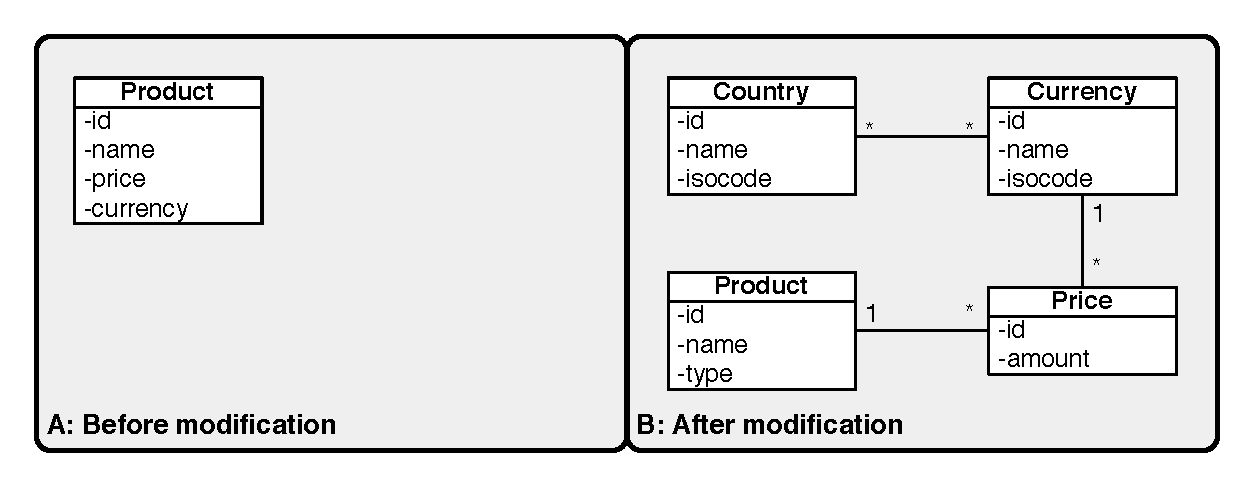
\includegraphics[scale=0.60]{images/ClassDiagramSample.pdf}
        \caption{Class Diagram Sample (before and after modification)}
        \label{fig:classDiagSample}
\end{figure}

With this example, we can clearly see that there are structural modifications but also data migration is required. There are some generic data and some contextual data. For example, the attribute type in the product class required to be updated depending on the data that are in the table at the time of the migration. This could be really tricky to update due to number of products already present in the table. Let assume that there is not a lot of data and that we could be able to write by hand the migration script. We can imagine that there is only ten products in the product table as the Fig. \ref{fig:classDiagDataBefore} shows the product table content before migration. The product tables contains vegetables and fruits (that will be stored later under type attribute). We did a simplification for the type attribute, we clearly imagine to create a class to store this data for cleaner approach of this data model. The script to create the table is shown on Listing \ref{list:classDiagSqlBefore}.

\begin{figure}[h]
        \centering
        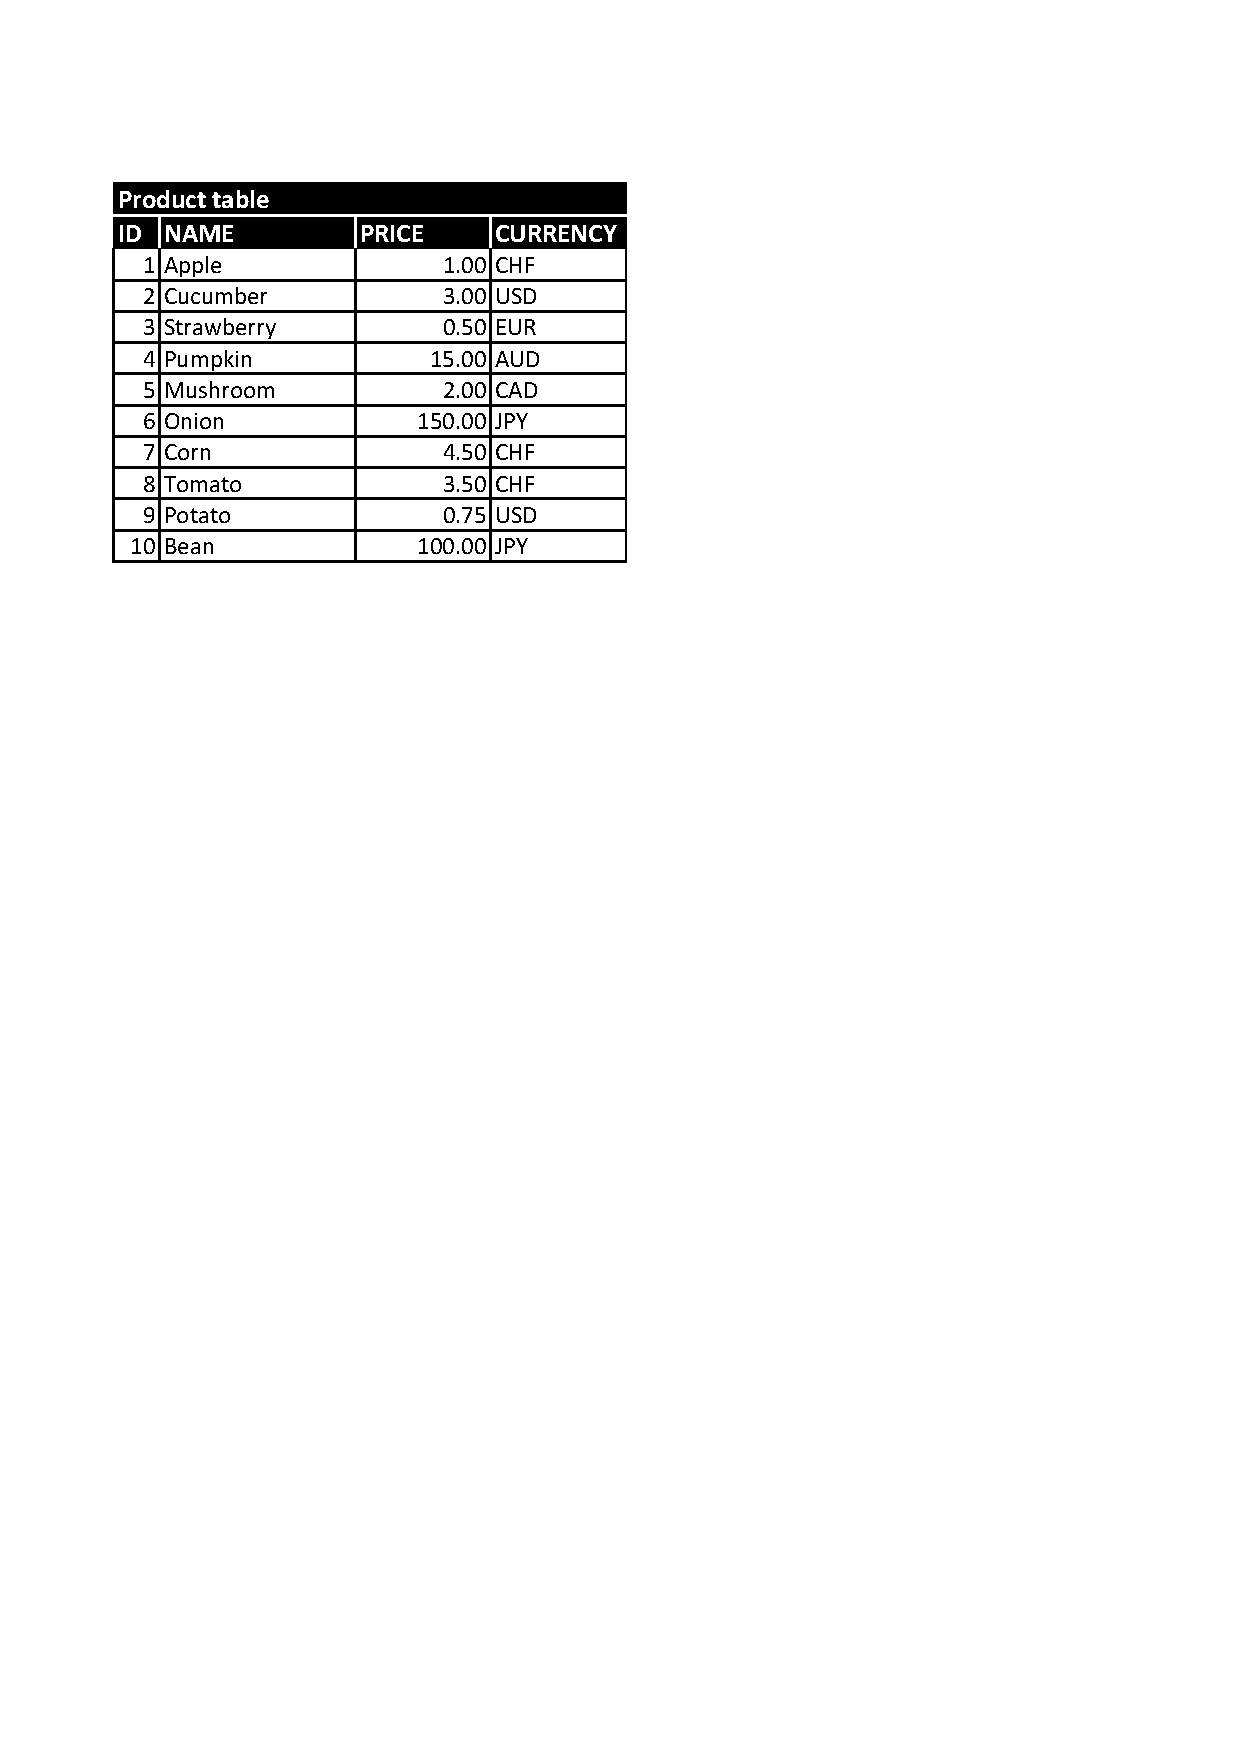
\includegraphics[scale=0.60]{images/ClassDiagramDataBefore.pdf}
        \caption{Class Diagram Sample - Data before modification}
        \label{fig:classDiagDataBefore}
\end{figure}

\lstinputlisting[label={list:classDiagSqlBefore}, caption={Class Diagram Sample - Schema before modification}, style={sqlStyle}]{sql/ClassDiagramSchemaBefore.sql}

Keep again an eye on the Fig. \ref{fig:genMigScriptSchema} and let's start with the migration writing. We know that the modification clearly implies a migration scripts. Does migration require multi steps? We are not sure at this step (or let assume that for the example). Which kind of migration is it? We have added classes and it implies schema update. So we are sure that there is a schema migration script. We also see that we need to add new data to fill the new tables implied by the migration. Is these data generic and/or infrastructural? Yes, they are for the Country and Currency tables. We also think about the price table that requires a major work to transform the data from Product table to Price table. At this cogitation, we discover that the type attribute must be filled depending on the data stored in the product table.

Finally, with this short example, we cover different the migration possibilities, schema, generic/infrastructural data and contextual data. At this stage, the developer must think about the migration ordering. It means that the queries must be ordered to be run correctly against the database that already contains data. Basically, we need to update the schema, adding new infrastructural data, migrate actual data and finally correcting/removing constraints/data. With our answers and reflexions, we clearly see that the script cannot be run in one part. We already know that we need to decompose our script into different parts. But first of all, let's go with the schema creation request. The queries could be seen on Listing \ref{list:classDiagMigrationStep1a}.

\lstinputlisting[label={list:classDiagMigrationStep1a}, caption={Class Diagram Sample - Schema migration - Step 1a}, style={sqlStyle}]{sql/ClassDiagramMigrationStep1a.sql}

At this step, we are ready to write the queries to populate the data that are generic/infrastructural. The countries and currencies are, in general, structural data that could be used in any environment. The queries (extract) could be viewed on Listing \ref{list:classDiagMigrationStep1b}. We also provide a query to extract the data for the three tables as we can view on Fig. \ref{fig:classDiagMigrationStep1bData}. We could discuss about the correctness of the hypothesis that the data are shared between different application deployment. We assume this is the case and that we use the same data in different deployments for this example.

\lstinputlisting[label={list:classDiagMigrationStep1b}, caption={Class Diagram Sample - Data migration - Step 1b}, style={sqlStyle}]{sql/ClassDiagramMigrationStep1b.sql}

\begin{figure}[h]
        \centering
        
\includegraphics[scale=0.60]{images/ClassDiagramMigrationStep1bData.pdf}
        \caption{Class Diagram Sample - Resulting data - Step 1b}
        \label{fig:classDiagMigrationStep1bData}
\end{figure}

We have also to insert the prices in the Price table before removing the columns. The queries could be viewed on Listing \ref{list:classDiagMigrationStep1c}. The queries could be done independently from the context. In any application deployment that has products, they are prices and currencies to convert/migrate. This job could be done by queries that are not dependents to the application deployment.

\lstinputlisting[label={list:classDiagMigrationStep1c}, caption={Class Diagram Sample - Schema and migration data - Step 1c}, style={sqlStyle}]{sql/ClassDiagramMigrationStep1c.sql}

So we have written the queries involved in the first step of the migration that add the new tables, add the constraints and add the data column to the existing entity. We also added the infrastructural data. Now, we have to place these queries to the right place. The Fig. \ref{fig:genMigScriptSchema-1} will help us to retrieve the migration number that we will use to situate the script into our migration process. We have simply to know where the modification is done. In our case, we suppose that the modification are done in working trunk directory of our versioned repository. Otherwise, we should get the migration number from the Branch/Release path and apply the rules for this situation. For the following paragraphs, we assume that the next migration number is 15.

\begin{figure}[h]
        \centering
        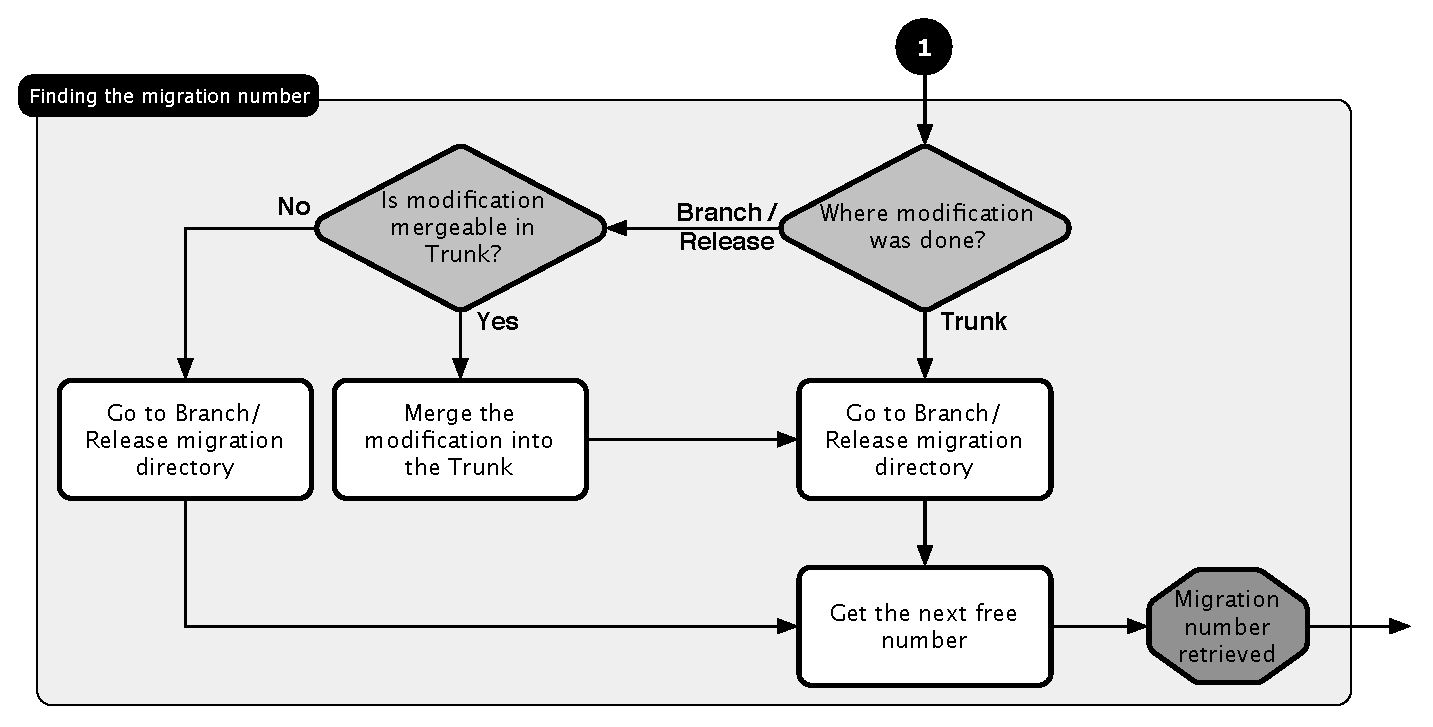
\includegraphics[scale=0.60]{images/mig-schema-gen-1.pdf}
        \caption{How to write a migration script schema - Subpart 1}
        \label{fig:genMigScriptSchema-1}
\end{figure}

When the migration number is retrieved, we can create the file to store the queries for the migration step. So, now, we need to follow the rules to build the migration name that could be viewed on Fig. \ref{fig:genMigScriptSchema-2}. Is there already a script for the migration (migration number we just previously retrieved)? In our case, we have only one script yet, so we need to build the name as "15.sql". A shortcut could be taken to build the script name because we already know that we will have another script for the same revision but for the example, we will strictly follow the rules.

\begin{figure}[h]
        \centering
        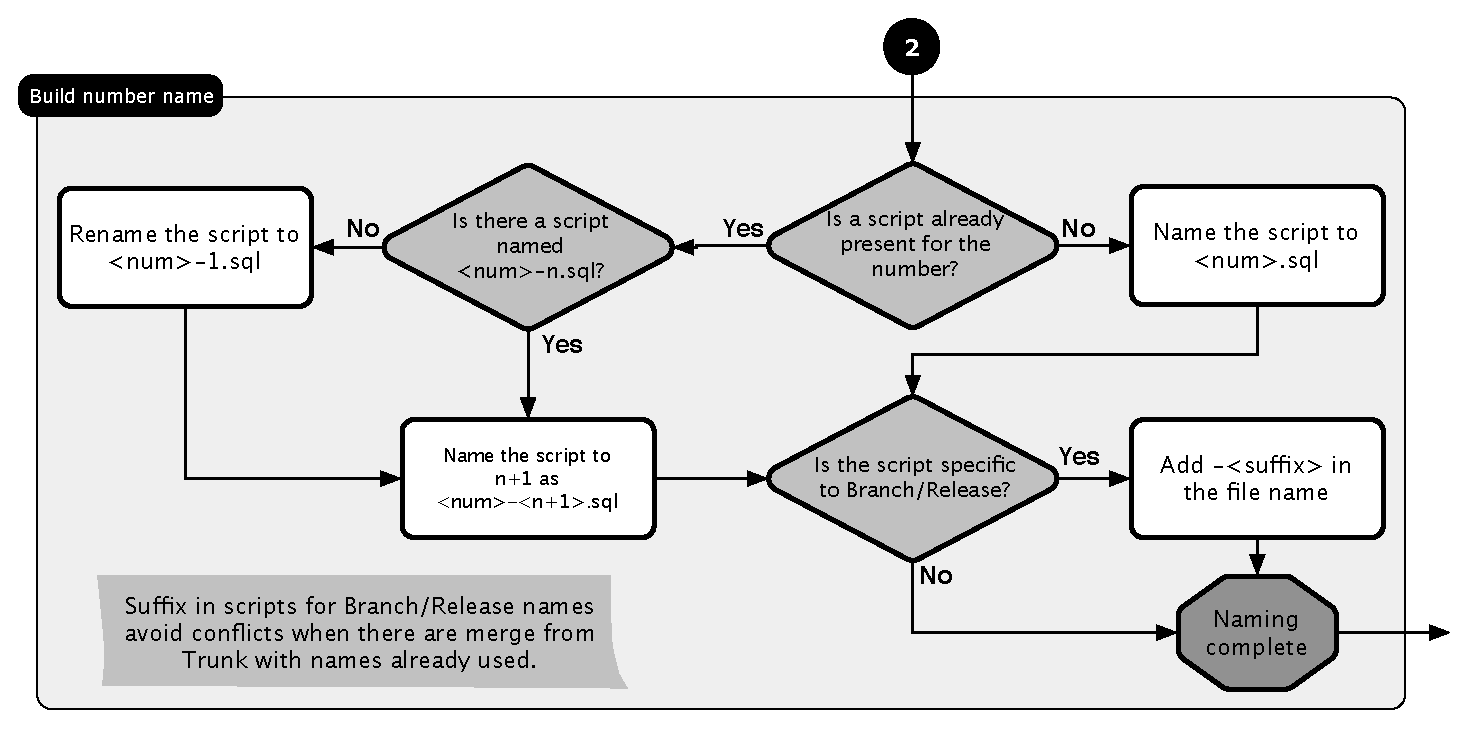
\includegraphics[scale=0.60]{images/mig-schema-gen-2.pdf}
        \caption{How to write a migration script schema - Subpart 2}
        \label{fig:genMigScriptSchema-2}
\end{figure}

In some situations, we need to add an information to influence the migration scripts ordering. Imagine that you did a correction into a release version in revision identifier 245 and you merged the correction in your trunk in revision identifier 253, you will have a migration script name like n.sql (or eventually n-<suffix>.sql if the correction was not planed to be merged into the Trunk). Some other scripts could be already present in the Trunk migration directory that you do not want they could be run before the script you just merged. For this reason, we introduce some annotations to help the script parts ordering. This mechanism is more largely used in the contextual scripts due to the naming conventions we used that is different from the migration number system. With @after and @before annotations placed in the comments of the migration part script, we are able to define precisely where a migration script must be run when the place is different from the normal one. The Fig. \ref{fig:genMigScriptSchema-4} shows how to use the annotations we have introduced. This system is designed to be used by some tools to help the concatenation of the different script parts. For the current migration script step, we do not need to specify any annotations for a special ordering.

\begin{figure}[h]
        \centering
        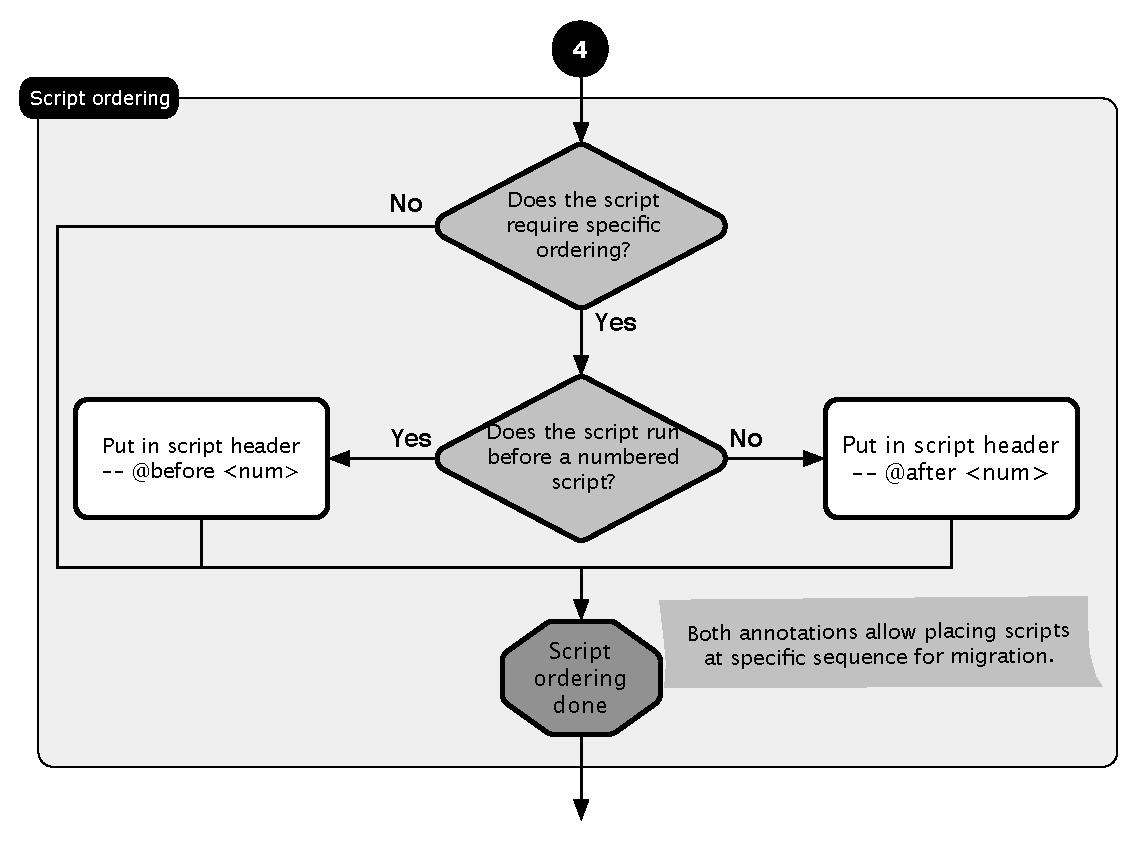
\includegraphics[scale=0.60]{images/mig-schema-gen-4.pdf}
        \caption{How to write a migration script schema - Subpart 4}
        \label{fig:genMigScriptSchema-4}
\end{figure}

We have finished one loop of the process to write a migration script entirely. We need to iterate, at least, one more time for the contextual data (data present in product table). So the Fig. \ref{fig:genMigScriptSchema} give us the next step to follow. This time we need to write contextual queries. The queries are not so complicated but depends entirely on the data present in the table product. We need to write the queries to add the type to each product. The Fig. \ref{list:classDiagMigrationStep2} shows an extract of the queries we have to write. For the example, the queries shown are specially simple and quite stupid, we can construct a better script that will be able to define the type of products based on the name with a lookup table for example but this kind of considerations is out of the scope.

\lstinputlisting[label={list:classDiagMigrationStep2}, caption={Class Diagram Sample - Migration data - Step 2}, style={sqlStyle}]{sql/ClassDiagramMigrationStep2.sql}

Now that we have the queries, one more time, we need to place the migration script at the right place. For that, we will follow the rules on Fig. \ref{fig:genMigScriptSchema-3}. We have to go to the right directory. First of all, we have, on the versioning repository, a dedicated directory to store the contextual migration scripts. We go into this directory. Then, we have to check if the directory for the environment we want to update is created, if not, we create the directory. By default, we use a dummy environment called "local" or "dev" to store the scripts before they will be adapted to the right environment. When the scripts are written, it is unusual that we already know for which environment we have to write the migration script and even if we know, until we have to migrate the environment, the data could change and the script could be not relevant. So, we will always create the contextual migration script into this dummy environment to be up to date with the migration monitoring. Generally, in multiple environment, the application deployment is not easy to follow because each environment could evolves differently. Each one could have a different version that requires a specific migration script based on the different migration script parts.

In the environment directory, we will check if a directory exists for the version deployed currently on the environment (called version from). If the directory does not exist, we will create it. And finally, we could check if a migration script already exist or not. If no, we will have a script name like "1-$<$FreeText$>$.sql" otherwise we will have "$<$LastNumber$>$+1-$<$FreeText$>$.sql".

In our example, we assume that we wrote the first contextual script for the dummy environment and version from which the next migration will be done. So, our script name will be like "1-AddTypeToProducts.sql". After that, we have just to go through the ordering rules to add an annotation to put the script just after the step one we just wrote before this one. We will add "-- @after 15-1" (Remember that the "-1" will come later due to the fact that the migration is split in two parts due to null constraint not addable when there are data with no default value).

\begin{figure}[h]
        \centering
        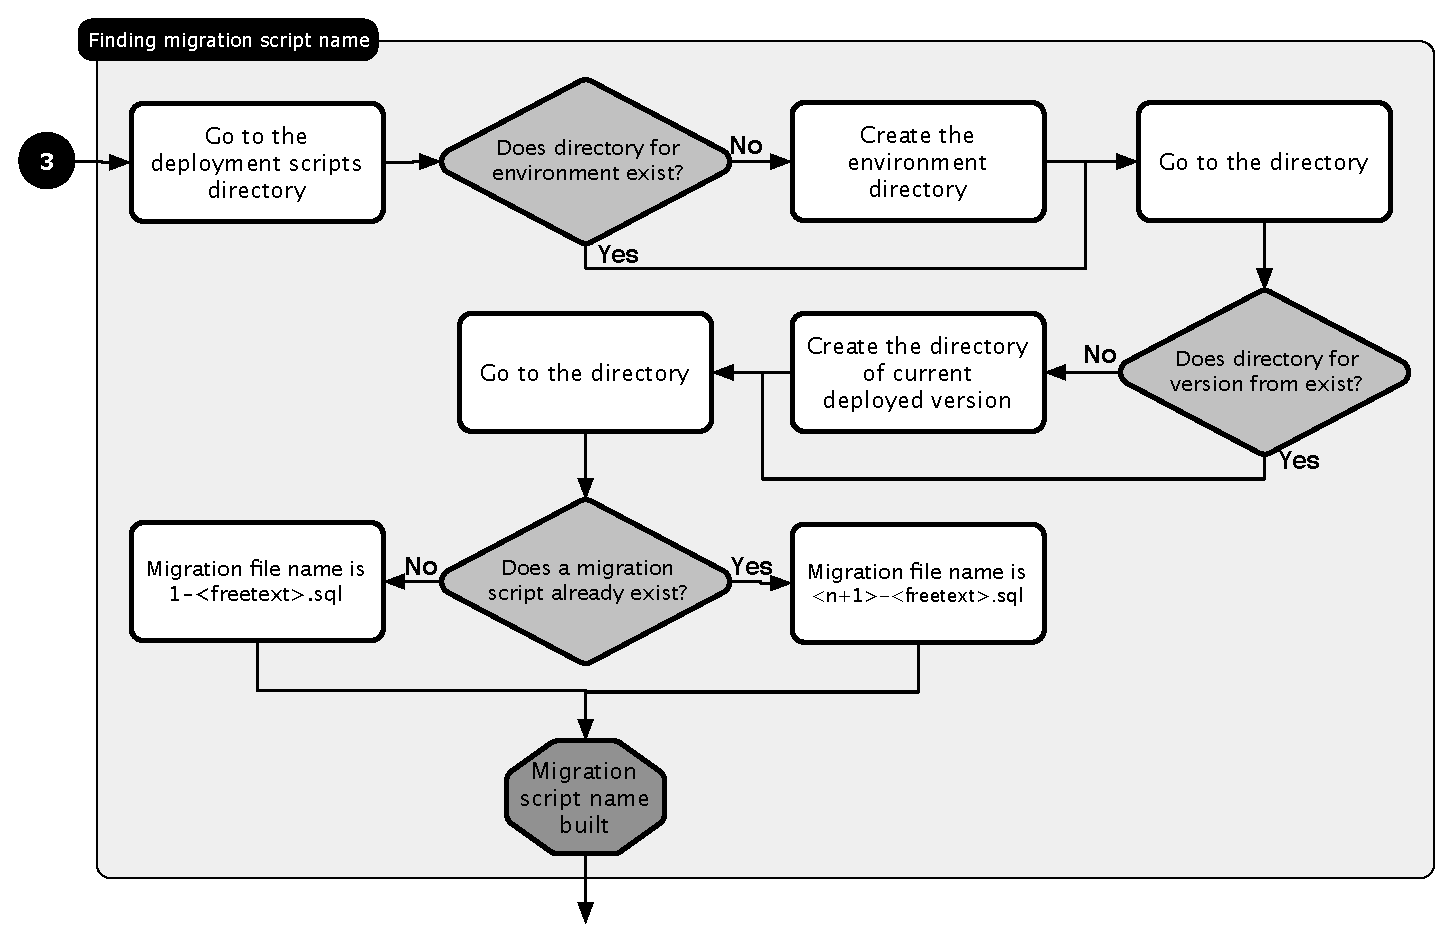
\includegraphics[scale=0.60]{images/mig-schema-gen-3.pdf}
        \caption{How to write a migration script schema - Subpart 3}
        \label{fig:genMigScriptSchema-3}
\end{figure}

Finally, we can conclude the migration with a final query to add the missing constraint on the column type on Product table shown on Listing. \ref{list:classDiagMigrationStep3} that we was not able to do before updating the Product data. So we will go through the rules diagrams again. When we have to find the name of the migration script step (based on the Fig. \ref{fig:genMigScriptSchema-2}) we see that there is already a script named "15.sql". So we need to rename the script to "15-1.sql" (as we already anticipated in the previous paragraph). When it is done, we will find the name for this step as "15-2.sql". That is all. We have finished to prepare the migration scripts. To finalize the migration writing process, we have just to commit the files into the versioned repository.

\lstinputlisting[label={list:classDiagMigrationStep3}, caption={Class Diagram Sample - Schema migration - Step 3}, style={sqlStyle}]{sql/ClassDiagramMigrationStep3.sql}

From now, we have a lot of migration scripts distributed across different files. When we will run a migration, we need to concatenate the files we want in the order required. This part is really tricky if it is done by hand. In the \autoref{sec:buildingScript} we provide a solution that could be used to automatize the concatenation of the migration scripts. The ability to have the different files allows building at any time, for any version, at any level a new application deployment. It becomes easy to deploy a new application in a new environment with the scripts that are able to prepare the database for the application.

\subsection{Tools}

To support the different processes defined previously, we need tools to help us. We provide some conceptual tool ideas that we could use.

\subsubsection{Code modification detection\\}

As we explained, we need the ability to detect code modification but especially modifications that have impact on the database schema and/or data. Generally, application code is such well organized that these modifications are easy to monitor with some addition to the versioning system in place. It is relatively easy to write plugins or scripts that add this logic to the versioning system with the ability to send emails with the potential matches triggered.

The persons in charge of code monitoring must have the information to quickly decide if a modification has an impact or not on the migration process. For that, the emails sent must contain at least the list of files impacted by code modifications. If the differences between two modifications is provided, the work to analyze what is implied in a migration is really more easy. The pseudo code \ref{pcode:monitoringPseudo} show a basic mechanism to monitor the code changes by a succession of filtering to include the path that have some interest and to exclude some of them in the result of inclusive filters. This allow getting only the files that are useful. The remaining code is present to prepare the result with the relevant information to help differentiate the database impacts.

\begin{algorithm}
	\caption{Code monitoring}
	\label{pcode:monitoringPseudo}
	\begin{algorithmic}[1]
		\State \tdefine{inclusiveFilter}{Path to include}
		\State \tdefine{exclusiveFilter}{Path to exclude}
		\State
		\State \Comment{Retrieve information from versioning system for the current version}
		\State \tdefine{changedFiles}{\Call{retrieveChangedFiles}{~}}
		\State
		\State \Comment{Apply filters to keep only relevant files}
		\State \tdefine{tempFiles}{\Call{applyInclusiveFilter}{\tvar{changedFiles}, \tvar{inclusiveFilter}}}
		\State \tdefine{remainingFiles}{\Call{applyExclusiveFilter}{\tvar{tempFiles}, \tvar{exclusiveFilter}}}
		\State
		\State \Comment{Prepare an email to send the code monitoring result}
		\State \Call{createEmail}{~}
		\State
		\State \Comment{Check if there are relevant files}
		\If{\tvar{remainingFiles} not empty} 
			\State \Call{addToEmail}{\tvar{remainingFiles}}
			\State
			\State \Comment{For all relevant files, extract the difference from previous modification}
			\ForAll{\tvar{changedFile} in \tvar{remainingChangedFiles}}
				\State \tdefine{result}{\Call{retrieveDifferenceFromPrevious}{\tvar{changedFile}}}
				\State \Call{addToEmail}{\tvar{result}}
			\EndFor 
		\EndIf
		\State
		\State \Call{sendEmail}{~}
	\end{algorithmic}
\end{algorithm}

As we seen, this conceptual tool is really simple to develop and put in place for basic requirements. It is also easy to improve and add additional monitoring. The only pre-requisite is to have a versioning system that allows to add plugins or hooks. If it is not the case, it is required to add mechanism to do this monitoring. For example, a scheduled monitoring everyday could be a solution if there is no way to integrate this tool in the versioning process.

\subsubsection{Migration info and statitics\\}
	\label{sec:migInfoAndStats}

When a migration is ready to be used, another requirements is to track the queries executed to allows gathering statistics as the duration of queries, the number of queries and such of things. In testing environment, it could allow to retrieve where a script loose to much time and which queries are costly. In addition, we can also store some data as the version from which we migrate and the version to which we migrate. We can store the versioning range identifiers for the migration.

For a relevant usage of these data, we need to store them directly in the application database in each environments. It offers a way to get information in real time at any time for any environments. In addition, if the application contains an admin interface, it could be integrated to it.

We have modeled the solution as shown in Fig. \ref{fig:migInfo}. Our solution is sufficiently generic that could be adapted to any use with small changes. We have one table that store the migration info (version from, version to, versioning start identifier, versioning end identifier, number of queries, duration, date start, date end). A second table that stores the metrics retrieved during the migration execution like number of inserts, updates and so on. The third table stores the different parts of a migration script with their duration. This table stores the details of migration execution that allows to know which script could be a bottleneck.

\begin{figure}[h]
        \centering
        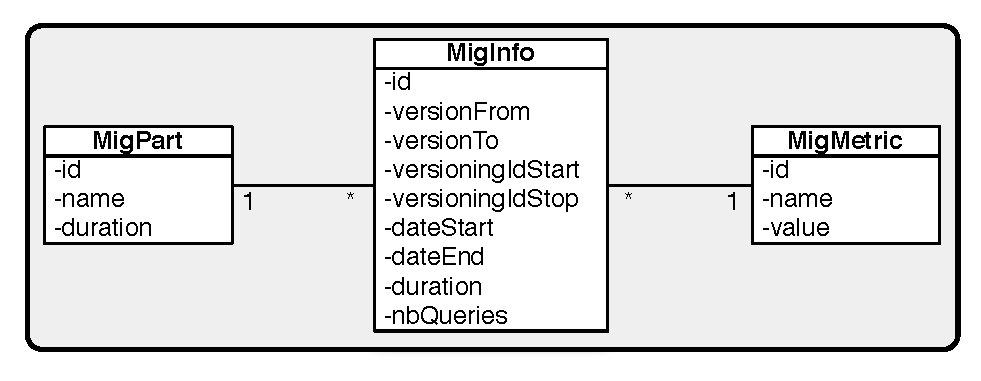
\includegraphics[scale=0.80]{images/MigrationInfo.pdf}
        \caption{Migration Info Model}
        \label{fig:migInfo}
\end{figure}

\subsubsection{Building tool\\}
	\label{sec:buildingScript}

To help the process to deploy a new application, we provide some algorithms to help to prepare the final script built from various migration parts. As we already discussed in \autoref{sec:rules}, we have added some logic to help the scripts ordering with annotations. These annotations could be placed in any script part. To build the final script, we need some information to retrieve the scripts and to do the correct sorting of scripts. We need to know the version from which we are migrating and also the version where we will be after the migration. The migration script number start and end are required to scope the migration script parts we will use. The environment is required to get the contextual script for the migration. Last but not the least, we need to know the application to migrate (and its database name). We need also to know if it is required to get the initial database creation with initial data population. What does it mean?

Up to now, we have discussed about migration but we need also to cover the first application deployment that is really similar with a major difference. In the development cycle, we do not want to manage migration scripts until it becomes required. We want to write migration scripts only when they are needed. For this reason, until the first deployment, we only write code without corresponding migration scripts. At the first deployment, we will create two files in the same way of normal migration scripts called "\_db\_creation.sql" and "\_db\_data\_init.sql". The first file contains the database schema corresponding to the application state at the deployment time. The second file contains the data corresponding to the schema and deployment needs. Eventually, some of data from this file must be placed in a contextual file as we already discussed.

With this approach, we keep agility to write code quickly until we have to deploy the application in a production environment. We could refactor any part of the application as we want without worrying about the consequences on migrations. At the first deployment, the application becomes "migration managed" application and needs to enter in the whole process we described. The both files are added at the final script beginning only if the building tool is asked for. We need to tell the tool if the application must be initialized or not.

Based on the different information gathered, we could build the runnable migration script. During the building process, we add some information as we have just discussed in the previous \autoref{sec:migInfoAndStats}. This data populates the different tables related to the migration information and statistics. The queries added are part of the runnable migration script. The pseudo codes \ref{pcode:buildingScript1}, \ref{pcode:buildingScript2}, \ref{pcode:buildingScript3}, \ref{pcode:buildingScript4} and \ref{pcode:buildingScript5} show how the building tool works.

In the pseudo code \ref{pcode:buildingScript1} we show how are the inputs required by the script tool to build the final migration script. We also get the migration part files directly from the versioning system to be sure to have the latest script parts. We initialize an empty list to store the resulting list of migrations to be include in the current migration. One part of the script, allows adding the initial database schema creation with initial data (like infrastructural and configuration data). This part is optional and could be configured when the script is called. 

\begin{algorithm}
	\caption{Builiding tool - Part 1 - Definitions}
	\label{pcode:buildingScript1}
	\begin{algorithmic}[1]
		\State \Comment{User inputs}
		\State \tdefine{versionFrom}{Get the version from}
		\State \tdefine{versionTo}{Get the version to}
		\State \tdefine{startNum}{Get the start number}
		\State \tdefine{endNum}{Get the end number}
		\State \tdefine{envir}{Get the environment}
		\State \tdefine{appName}{Get the application name}
		\State \tdefine{appDbName}{Get the application database name}
		\State \tdefine{initialize}{Get the application initialized or not}
		\State
		\State \Comment{Interaction with the versioning system}
		\State \tdefine{migrationFiles}{\Call{retrieveFromVersioningSystem}{\tquote{migration files}}}
		\State \tdefine{contextualFiles}{\Call{retriveFromVersioningSystem}{\tquote{contextual migration files}}}
		\State
		\State \Comment{List to store the migration parts in a ordered way}
		\State \tdefine{orderedList}{\O}
		\State
		\State \Comment{Add initial scripts if required}
		\If{\tvar{initialize}}
			\State \Call{addAtEnd}{\tvar{orderedList}, \tquote{\_db\_creation.sql}}
			\State \Call{addAtEnd}{\tvar{orderedList}, \tquote{\_db\_data\_init.sql}}
		\EndIf
		\algstore{bkbreak}
	\end{algorithmic}
\end{algorithm}

The second part of the building tool shown on pseudo code \ref{pcode:buildingScript2} manage the migration script parts that could be applied on every deployments. We assumes that the list of files analyzed is already sorted in the chronological order of numbering info. For each file, we check that is or not in the scope of the configured migration. We keep only the ones that are in the scope. For the others, we check the annotations in the files to see if they could be integrated to the current migration or not.

\begin{algorithm}[h]
	\caption{Builiding tool - Part 2 - Migration files}
	\label{pcode:buildingScript2}
	\begin{algorithmic}
		\algrestore{bkbreak}
		\State \Comment{Analyze migration files}
		\ForAll{\tvar{migrationFile} in \tvar{migrationFiles}}
			\State \tdefine{migrationNumber}{\Call{getMigrationNumber}{\tvar{migrationFile}}}
			\State
			\State \Comment{File is in the range of scripts wanted}
			\If{\tvar{migrationNumber} $\geq$ \tvar{startNum} \&\& \tvar{migrationNumber} $\leq$ \tvar{endNum}}
				\State \Call{addAtEnd}{\tvar{orderedList}, \tvar{migrationFile}}
			\ElsIf{\Call{containsAnnotation}{\tvar{migrationFile}}}
				\State \Comment{See pseudo code \ref{pcode:buildingScript4}}
				\State \Call{analyzeFile}{\tvar{orderedList}, \tvar{migrationFile}, \texttt{False}}
			\EndIf		
		\EndFor
		\algstore{bkbreak}
	\end{algorithmic}
\end{algorithm}

In the third part shown on pseudo code \ref{pcode:buildingScript3}, we analyze the contextual migration parts. The mechanism is pretty the same as the previous analysis. The difference remains in the analyze file procedure that trigger if the file is contextual or not. We will discuss about that a little later.

\begin{algorithm}[h]
	\caption{Builiding tool - Part 3 - Contextual files}
	\label{pcode:buildingScript3}
	\begin{algorithmic}
		\algrestore{bkbreak}
		\State \Comment{Analyze contextual files}
		\ForAll{\tvar{contextualFile} in \tvar{contextualFiles}}
			\State \Comment{See pseudo code \ref{pcode:buildingScript4}}
			\State \Call{analyzeFile}{\tvar{orderedList}, \tvar{file}, \texttt{True}}
		\EndFor
		\algstore{bkbreak}
	\end{algorithmic}
\end{algorithm}

Finally, when the ordered list of migrations files is ready, we could build the final script with some additions for the migration process. In the pseudo code \ref{pcode:buildingScript4} we show how the final script is built. We prepare a file with a header that contains a part that we call manifest. This manifest contains all relevant data used to build the final script and to have tracking data. For example, we will store the version from and to, versioning identifiers, creation date and the list of migration script parts we have in the final migration file. We also prepare some statements for statistical purposes. After that, for each file we add in the final one, we add some comments to create sections in the file to be userfriendly readable. Each migration part is separate by a header and footer that scope the migration part in the final file. The listing \ref{list:resultingFile} shows a result that could be produced by the building tool. We also add some metric queries for the current migration script (for example, we triggered the time duration of the current migration script part into the whole migration script. And finally, we add a final footer that contains the queries to populate the different migration tables in the application database.

\begin{algorithm}[h]
	\caption{Builiding tool - Part 4 - Build final script}
	\label{pcode:buildingScript4}
	\begin{algorithmic}
		\algrestore{bkbreak}
		\State \tdefine{finalScript}{\Call{createFinalFile}{~}}
		\State
		\State \Comment{Populate final file with statistical queries}
		\State \Call{addFileHeader}{\tvar{finalScript}}
		\State
		\State \Comment{Iterate in the chronological order}
		\ForAll{\tvar{file} in \tvar{orderedFile}}
			\State \Call{addHeader}{\tvar{finalScript}, \tvar{file}}
			\State \Call{addPreMigrationPartMetricQueries}{\tvar{finalScript}, \tvar{file}}
			\State \Call{addScript}{\tvar{finalScript}, \tvar{file}}
			\State \Call{addPosMigrationPartMetricQueries}{\tvar{finalScript}, \tvar{file}}
			\State \Call{addFooter}{\tvar{finalScript}, \tvar{file}}
		\EndFor
		\State
		\State \Call{addFileFooter}{\tvar{finalScript}}
		\algstore{bkbreak}
	\end{algorithmic}
\end{algorithm}

\lstinputlisting[label={list:resultingFile}, caption={Final migration script example}, style={sqlStyle}]{sql/migrationResult.sql}

The procedure to analyze the files to know if we need to keep them or not. For simplifications, we do not manage correctly the problem of transitivity. We mean that we do not follow the annotations across the script parts. If a script is annotated to be before one another script that also contains an annotation defining to be before one more script, we will lost the first annotated script with the pseudo code \ref{pcode:buildingScript5}. Some other case of transitivity are covered. It is relatively easy to modify our pseudo code handle this use case but the pseudo will become more complex to read. So, we retrieve the annotation number and the annotation type (after or before). If the annotation is in the range we have specified for the migration or the annotation is already in the range, we will add the file to the list. We have also to check if the list already contains a file for the annotation number, if this the case, we simply add the file after the one found otherwise we just add the file at the correct place relative to the annotation number. For the contextual scripts, we also check that if there is no annotation, we simply add them to the end of the list in the goal to manage them manually. The building tool could provide some mechanism to move manually some scripts before building the final script.

\begin{algorithm}[h]
	\caption{Builiding tool - Part 5 - Procedure to analyze annotated script parts}
	\label{pcode:buildingScript5}
	\begin{algorithmic}[1]
		\algrestore{bkbreak}
		\Procedure{analyzeFile}{\tvar{orderedList}, \tvar{file}, \tvar{contextual}}
			\State \tdefine{anNumber}{\Call{getMigrationNumberFromAnnotation}{\tvar{file}}}
			\State \tdefine{anType}{\Call{getAnnotationType}{\tvar{file}}}
			\State
			\State \Comment{Check if the annotation implies to add the file}		
			\If{(\tvar{anNumber} $\geq$ \tvar{startNum} \&\& \tvar{anNumber} $\leq$ \tvar{endNum}) \textbar\textbar~\tvar{anNumber} in \tvar{orderedList}} 
				\State \tdefine{fileFound}{\Call{findFileByNumber}{\tvar{orderedList}, \tvar{anNumber}}}
				\State
				\State \Comment{Check the file exists in the list}
				\If{\Call{isNotNull}{\tvar{fileFound}}}
					\If{\tvar{anType} = \tquote{@after}}
						\State \Call{insertAfter}{\tvar{orderList}, \tvar{fileFound}, \tvar{file}}
					\Else
						\State \Call{insertBefore}{\tvar{orderList}, \tvar{fileFound}, \tvar{file}}
					\EndIf
				\EndIf
			\ElsIf{contextual}
				\State \Comment{Add the script for manual processing}
				\State \Call{addAtEnd}{\tvar{orderedList}, \tvar{file}}
			\EndIf
		\EndProcedure
	\end{algorithmic}
\end{algorithm}

\section{Data migration categorizes and risks}
	\label{sec:risks}

The perspective of a data modification is always accompanied by a risk. The risk could be a data loss, a data corruption, a technical failure, a change that brings integrity errors, a change that makes the application no more compatible with the data schema, a missing change and so on. We see they are a lot of different risks. In addition of the risk, the complexity is another factor to consider in a migration. The complexity define the difficulty to write some scripts and the impact they could have. It is quite difficult to be absolute with this axis. In general, the complexity could greatly vary depending on the query types but also from the query purposes.

One another aspect to consider is the technologies used by the application to retrieve and manipulate the data. Depending of these technologies, some modifications have a lower impact or no impact than others. For example, adding a column to a table with no constraint (allows null values, duplicates and so on) will be negligible. The application can use the schema with this additional column without any influence but any insert will produce a null field in the row. This is definitively not a good practice.

We must to be careful about the database server used because some of them does not support transactions for all the query types. For example, MySQL\cite{mysql} server does not support transactions for DDL\cite{ddl}. All schema modifications could not be rolled back automatically by the database server. This could have a real impact on migrations. Having queries with transaction supports mixed with no-transaction queries does not make any sense. If it fails during the migration, we have to rollback all the queries or to find a way to retrieve the state of the error and start again from there. This is not a trivial task.

Our experience allows us to categorize the migration by type of changes and complexity and risk. On the figure \ref{risksTable}, you can see our appreciation of the different migration types.

\begin{figure}[h]
        \centering
        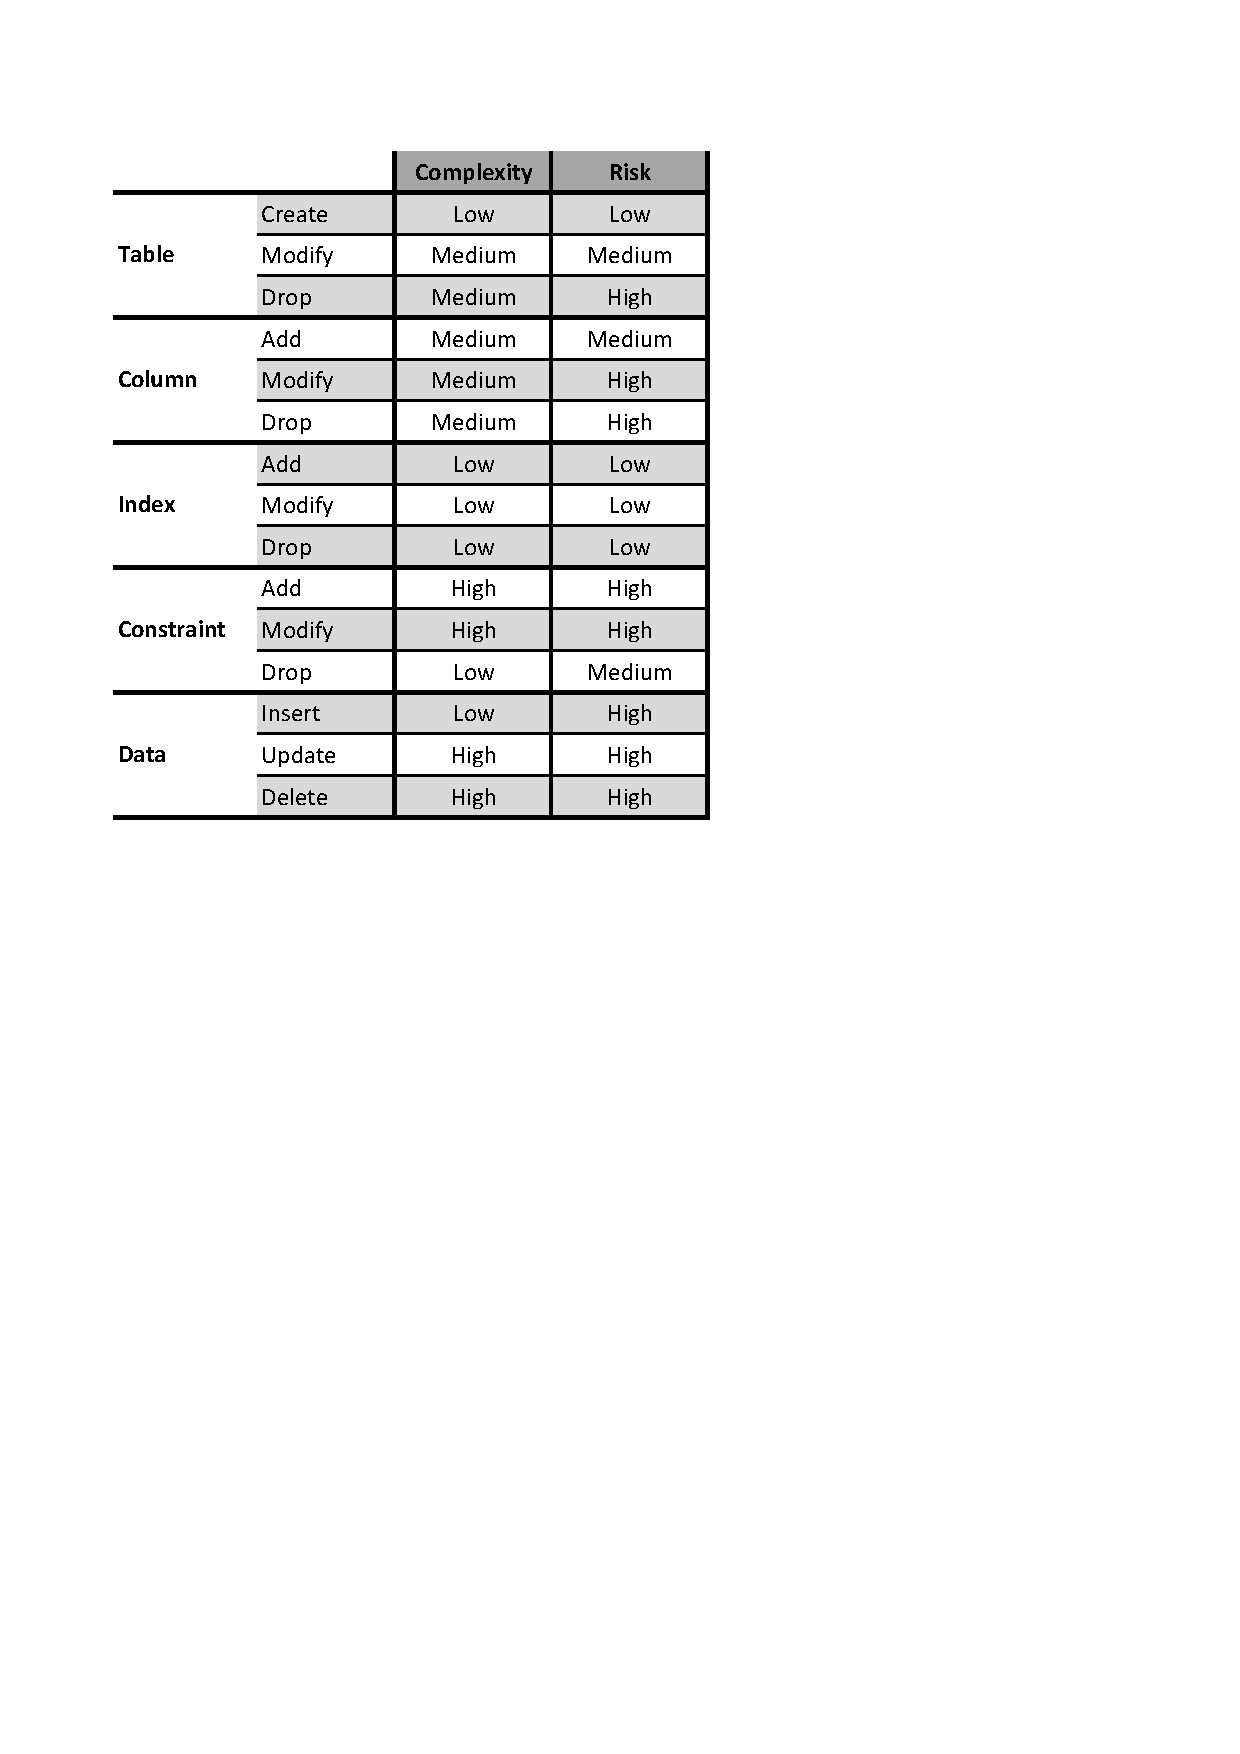
\includegraphics[scale=0.7]{images/risks.pdf}
        \caption{Risks table}
        \label{risksTable}
\end{figure}

\subsection{Table migration}

\subsubsection{Create a table\\}

Create a new table is not a big risk for both axis because the table is there to add a new feature. But you have to keep in mind that adding a table could cause some side effects. In fact, when you add a table, you need probably to populate it with data corresponding to the data you already have in your database. This part could be really tricky because you need to create data based on what you have. This part could be risky or not, it really depends on what is the purpose of your table. There is no absolute rules to define if the addition of a table implies a low or high risk on your business.

\subsubsection{Modify a table\\}

In this case, a modification means to rename the table. The complexity is medium because the command to change the name is quite easy to write, to test and validate. The risk is limited because you only change the name of your table and you would not alter the table content. So you do not risk to loose or corrupt data. If the change is not managed correctly, you risk to have an interruption of service during the time that your application is not mapped to the correct table name.

\subsubsection{Drop a table\\}

Dropping a table is quite easy from complexity point of view. The command is easy to write and test like the renaming command but from the risk point of view it is clearly a major risk. You need to have the insurance that dropping a table is ok and will not produce a non-wanted data loss. You maybe have to think about an archiving procedure before dropping the table and erasing all its content.

\subsection{Column migration}

\subsubsection{Add a column\\}

As we have already briefly discussed, adding a column to a table is not necessary risky. In general, this is not but sometimes, the nature of the column will imply a risk due to the fact that you need to fill in the column with data. In this situation, you can encounter two cases. The first is that the data can easily deduct or filled with default value, the second one is more complicated because you need to calculate the data or to fill the empty field with data based on a the context of the data already present in the database. The second case is more risky and complex than the first one.

It is difficult to choose a risk level or complexity level for this kind of migration because it really depends on the data that the column represent. It could be a low risk as it could be a high risk. Filling the column could imply a more complex procedure if the data to fill are calculate or deducted from the data context.

\subsubsection{Modify a column\\}

Technically, modifying a column is not complex. There are several kind of column migration. You could have to rename, change data type, modify the encoding. Renaming a column is probably the lowest complexity you could have in a migration while a data type change is a bigger complexity. When you change a column type, you risk to truncate your data, loss precision when float are stored and other strange behaviors that will corrupt your data. Changing the encoding has the same kind of risk as the type change.

\subsubsection{Drop a column\\}

Dropping a column is specially risky for the due to the fact you can loose data if you manage the modification incorrectly. You have to take care about the impact of the database. For the complexity point of view, removing a column is not a problem if in the application there is no more reference to this column. Your application can live with a small overload of data implied by a column not dropped that normally must. The complexity could be higher when the column is a foreign key to another table. This kind of modification are always more complex to manage.

\subsection{Index migration}

The index manipulation is probably the lowest risk in database migration. The queries are quite simple and do not imply data directly. We mean that the data stored in your tables remains the same when you manipulate indexes. One risk is on the performance point of view when you add a non-relevant index or when you drop a crucial index that improve your performance.

One thing that could happen is that a migration of your data required an index that is not present. An index missing could implies a very big problem in terms of performance. Some migration that requires few minutes to be executed, could in case of index missing take tens of minutes to be executed with a downtime of your application or service for this time. When a migration is required, taking a look of the indexes must be really useful to avoid lack of performance.

\subsection{Constraint migration}

The constraint migration is a category that implies more subsequent migrations. In general, you need to prepare your database when you add a constraint, you have to correct your database when you remove or update a constraint.

\subsubsection{Add a constraint\\}

Adding a constraint is not easy. It really depends on your data you already have in your database. For example, if you add a constraint that check if a value is unique across a table, you need to check before adding the constraint if there is no duplicates in your data otherwise you will not be able to add the constraint. In this case, you have to decide what to do with duplicates. This is the part that is not easy. Depending the situation, you will not be able to manage easily the duplicates.

\subsubsection{Modify a constraint\\}

As the same as adding a constraint, the modification of one constraint implies the same kind of troubles. You will have to analyze carefully the data you manipulate through your constraint modification to know what to do with them. It is really dependent of the context.

\subsubsection{Drop a constraint\\}

We think that dropping a constraint is not a big complexity because, in general, this relax the constraints imposed to the data. On the other side, risk is quite low, removing a constraint could cause some insidious long terms errors. You have to clarify why a constraint must be removed. You have to guaranty that your application will ensure some correctness of your data. For performance aspects, removing the constrain will be useful but will imply a major risk on your data and especially if your application is not robust or when you have more than one application against the same database. Some data corruption could happens and will not be seen for a while.

\subsection{Data migration}

On all migration category, the data manipulation is the most risky and complex. You can easily corrupt the data in your database without perceiving any problems before a while. Some corruption will appear only after a certain time when your application run into some border case for example. In this case, the correction of the data could be really tricky. The complexity comes from the data themselves. Depending on the data, your migration could be easy or really tricky. You need to know exactly your data to update them.

\subsubsection{Insert data\\}

Inserting data is quite easy for complexity aspects but could be risky. You can easily imagine a case that when you insert new data, you expose them to the wrong public if your system offers a security filtering of your data. You can also exchange text column in a request without an error at the time of your migration but the final customers could see strange texts or strange behaviors that are not easy to detect.

\subsubsection{Update data\\}

When an update is run in a database, if the query is wellformed but semantically erroneous, you risk to update more data than you expect. This is a major risk. Imagine that you have a table with a field name that is unique and you have no constraint on the table to enforce that. Running a query that update this name without specifying a restricting clause to only the record you want to update could cause an update on all your records. If the application relies on name are unique, the application will not be able to handle the data correctly if the records' name are all the same. This is a school case, so one more concrete example. Imagine you have a table to manage Internationalization with a name and a string corresponding to the name. If an update is run without specifying the specific record where to update the string, all the records will see their value changed. In this case, all the translations will have the same wording that is really bad for the final user.

\subsubsection{Delete data\\}

The high risk in deleting data is principally the loss of data that is really critical for a company. In regards of the data, the application could be totally broken after a data deletion. The complexity could be quite high due to the references to other tables. Especially when you have circular references (not a best practice at all).
\section{Case Study: Application of the Framework at Lotaris}

The main business in Lotaris SA is the license management. We develop a solution to manage and provide license management for ISV (Independent software vendor). In our solution, we develop different server side components shown on Fig. \ref{fig:globArchi}. We based our developments on Java technologies and especially Java Enterprise technologies where we use JPA\cite{jpa}.

\begin{figure}[h]
        \centering
        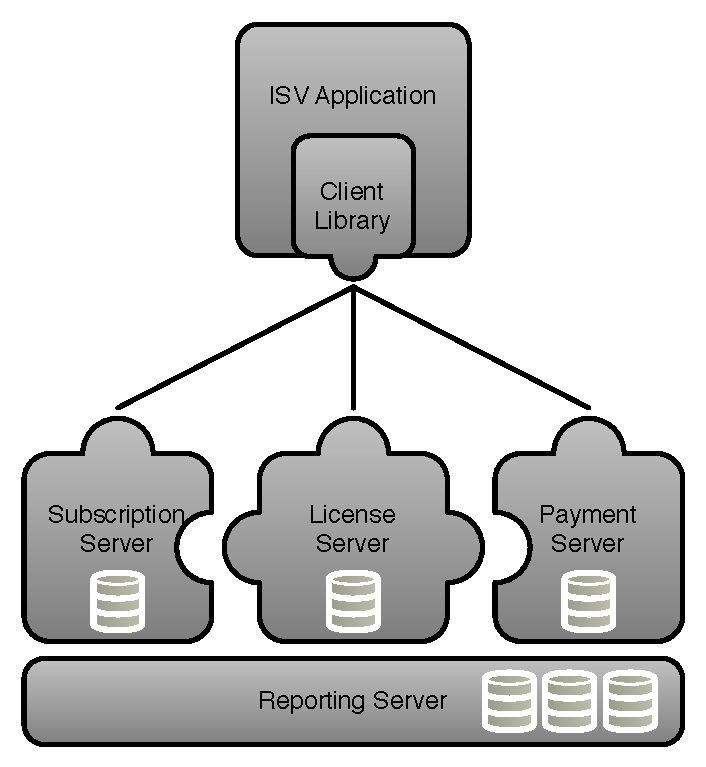
\includegraphics[scale=0.5]{images/archi-glob.pdf}
        \caption{Global architecture}
        \label{fig:globArchi}
\end{figure}

In such context, we use JPA as an ORM that offers an easy way to develop the data binding between the database and the application. As we have started from zero, we have used the ORM from the application to the database. This approach implies some flexibility in terms of developments and relies on the capability of the ORM. We do not need to manipulate directly SQL commands directly due to the mechanism offered by the abstraction of JPA. This is really appreciable but we loose some controls on specific behaviors and performance aspects. We have the possibility to write native SQL but we avoid this solution as much as possible. We tried to write only data access through the API offered by JPA. In other hand, when the configuration is done properly, the database schema is auto-generated and deployed when the application is deployed in the application server. 

Like every great technology, there are several disadvantages like the fact that you do not realize directly that your modification of the code could occur a database change. Adding an attribute to a data model class will produce a new column on the database schema. The code is more easy to change than the database. So, we specially need process to trigger these modifications as we presented in the \autoref{sec:def}.

At Lotaris, we are using SCRUM methodology. This methodology is part of Agile methodologies. We organize our work in sprints of two-three weeks between each release. It means that each sprint we have a new version with potentially database modifications. The Agile methodologies are organized around the possibility to evolve applications to the market needs, to change the user requirements as soon as possible in the development cycle. In general, it always means feature modifications, domain model modifications and so on. These abilities allow mitigating risky modifications and evolving before the application development is too far. One of the main aspect is the fact to build an application as simpler as possible and refactoring only when it is required. Following this way means a lot of modifications that will impact our databases.

Our goal is to keep this methodology for the agile ability. For that, we absolutely need processes and tools to help us in the development cycle. We need to keep easiness of development and fast deployments. We expect everyone is able to write some basic queries (DDL, SQL, ...) or more complex with the help of senior developers. As we discussed in \autoref{sec:def:developer}, each developer is responsible for his modifications and their impacts. It does not mean nobody will help developers to write tricky queries. 

When we started the work on the migrations, we had no clear processes or tools. We started to build iteratively each piece that compose our framework. As we have production imperatives, we had to deal with the schedules and what we could do to improve our migration work. For now, we only deployed in production one of our components with the shared code.

\subsection{Initial deployment of an applciation}

The first deployment of an application is pretty easy. We start from scratch and database schema and data are quite scoped. It is easy to prepare the release based on testing data and infrastructural data. Other required data are quite easy to insert at the beginning. With few SQL scripts, we create the initial stage of an application. The application has no business data and starts its production lifecycle. From this point, the application needs well done migrations each time the application evolves. For these reasons and ones we already discussed, we need to start to think about the migration process. Otherwise, we encounter the same problems that we had when we did our first migrations.

\subsection{Migration pre framework}

When we prepared our migrations, we started to ask us some questions to organize the data migration part. The application did not contain too much model modification that required data migration. It was quite easy to follow modifications and to write the relative migration scripts. At this stage, we already put in place some rules like the separation between queries that could be applied to all environment than the ones that could not be applied on all environments. But all the stuff done at this stage was really handy and specially difficult to handle correctly.

Our experience from these migration were quite awful. We did all by hand and we had no confidence in our migrations. All was done in urgent way with the consequences that could happened. We had done these migrations in pair programming to enhanced the efficiency of the tasks required for the migrations. We had cross-checked our scripts and validated them in a local environments. It was particularly difficult to retrieve the changes and to write the relative scripts. One developer was in charge of the migration. He had to retrieve the modifications and to write the missing scripts with the help of other developers. He had to compare database schemas manually to be sure no modification was missing.

We use Subversion\cite{subversion} as our versioning system. It is a centralized versioning system with a revision numbering system that is incremental. During this first migration, we used the revision number to name our migration script. This trick allows us following the modification by the script file name. We go through all the revisions implied in the migration to analyze and write the migration scripts. The \autoref{fig:StatMig1} shows the information about one of our migrations. The statistics were gathered directly from migration script. We had separated the scripts between our shared component and application component. Each component had its own directory that contains the migration scripts. For the script that must be run only on the specific production environment, we stored them in a specific directory without any structure. We stored the scripts by topics.

\begin{figure}[h]
        \centering
        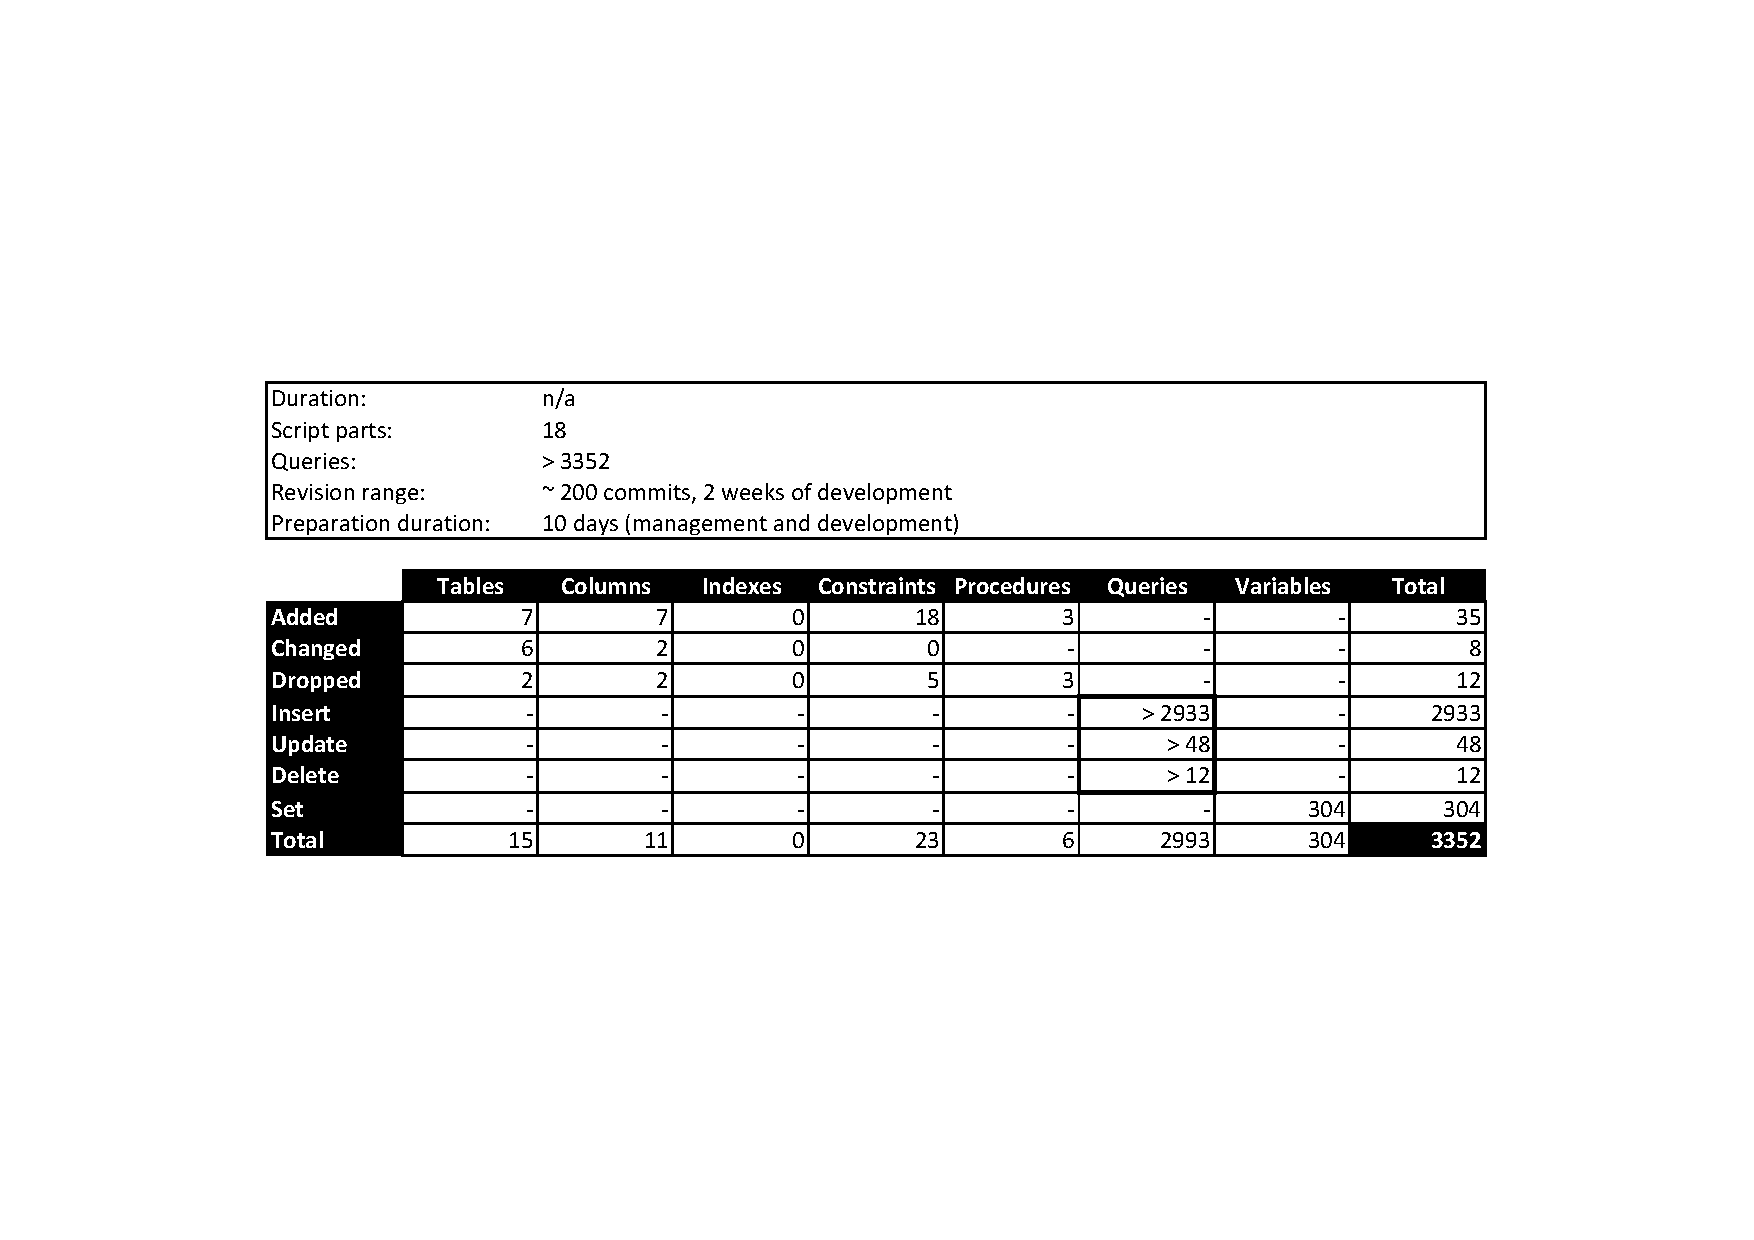
\includegraphics[scale=0.65]{images/Statistics_mig1.pdf}
        \caption{Statistics for a sample migration before introduction of framework}
        \label{fig:StatMig1}
\end{figure}

As we shown on the \autoref{fig:StatMig1}, the statistics are quite interesting. We see that we have run more than 3300 queries. This number is approximative due to the fact we use stored procedures. The methodology to gather the statistics was just to count the statements in the script we run. It means, in the case of stored procedures, that we had count only one time each statement written in the script. It is clearly a naïve approach. We have only the minimum of insert, update and delete queries. We had not monitored the time that the migrations took in our production environment. The way we handle the statistics is clearly a point of improvements. 

The preparation of final scripts were done by hand. It means that each script part was added manually to final scripts. All the preparations took approximatively ten days with a lot of work done by hand. A lot of repetitive tasks that encourage errors and delays. We clearly saw that we needed more structure to handle correctly our migrations. These migrations were quite anarchic.

\subsection{Migration with a basic framework}

For these migrations, we had the time to put in place some concepts, process and tools. We have created a tool to automatize the creation of the final script from the different script parts. It allowed to save time and manual handling. By the way, it drastically reduced the risk of errors and missed scripts. We had introduced a basic process to help the developer to write migration script parts. The process we used for these migrations are shown on \autoref{fig:MigSchemaGenMainPremise} where it is a premise of the actual process we use. Basically, the process is just a formalization of the tasks we instinctively did. At this time, we did not have any documentation that each developer can use to write his scripts. Each developers asked the migration manager to know what and how to do the required tasks to prepare migrations.

The tool we wrote is a script in Ruby\cite{ruby} that checkout the scripts from our subversion repository. Then, the different files that are involved in the migrations are concatenated together in the chronological order. From there, the script allows to use some commands to manually reorder the script parts to get the final sorted script. This script is a previous version of the pseudo code presented in \autoref{sec:buildingScript}. The usage of this tool required a lot of knowledge about the script parts for the correct ordering. We needed to know where to put each file due to the basic algorithm to auto-sort the migration parts.

\begin{figure}[h]
        \centering
        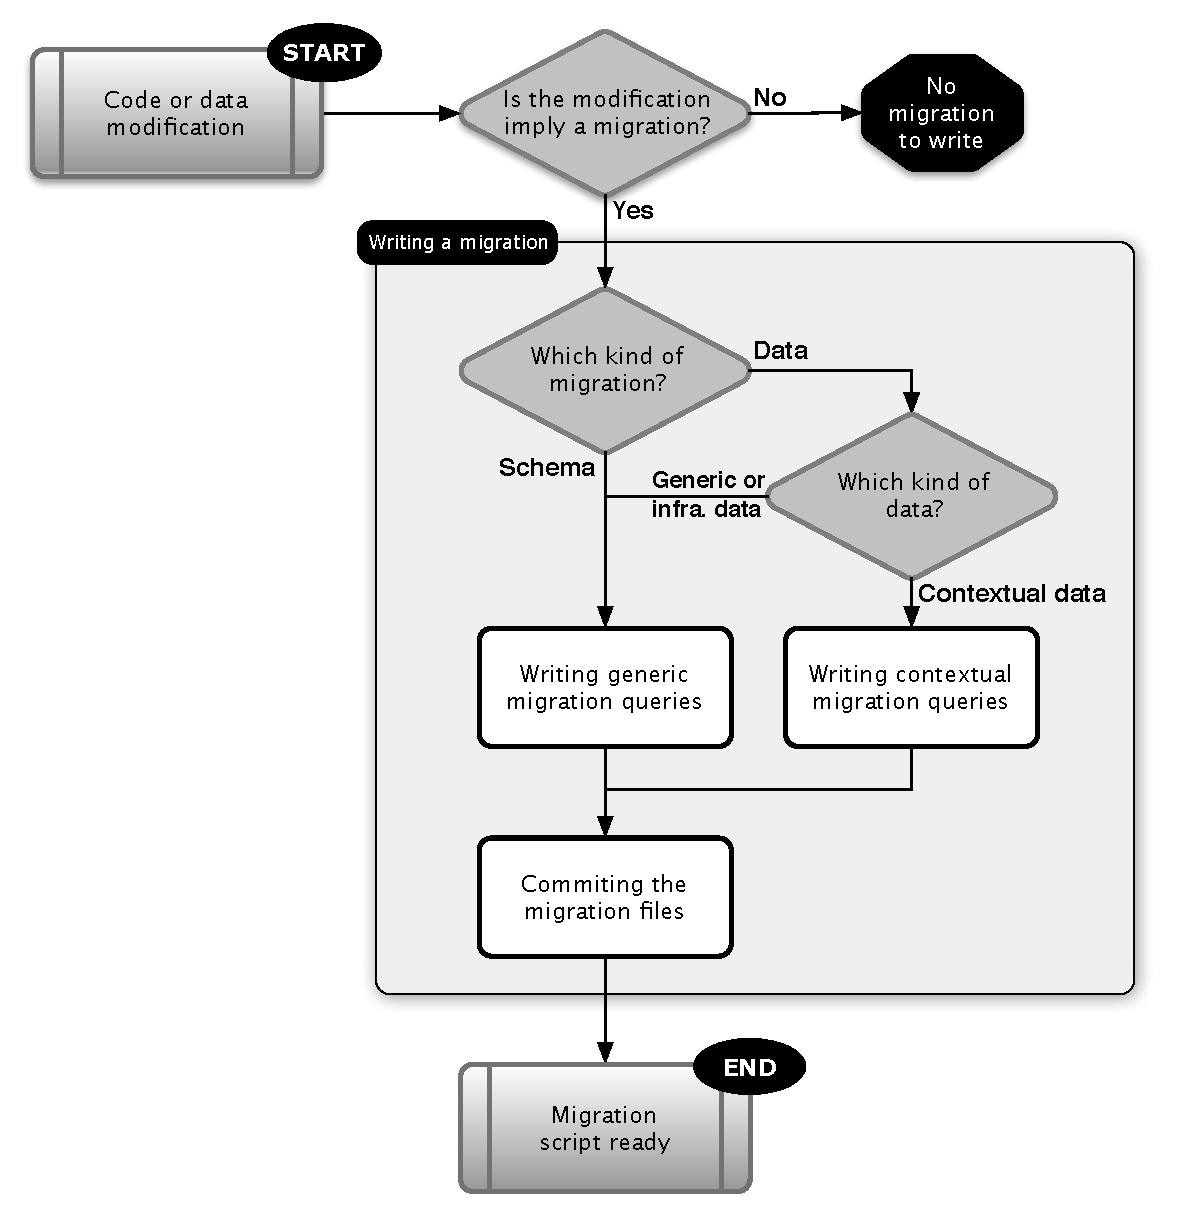
\includegraphics[scale=0.50]{images/mig-schema-gen-main-premise.pdf}
        \caption{Premise migration process}
        \label{fig:MigSchemaGenMainPremise}
\end{figure}

Unfortunately, we were not able to follow regularly the modifications done with an impact of database schema. We accumulate some delays in the monitoring of the modification and in the script writing. We tried to write the scripts each time it was required without success due to the unformalized process. In addition, the rules were not so clear and some mistakes were done in the writing process. Some queries that are contextual were written in generic migration files and vice versa.

\begin{figure}[h]
        \centering
        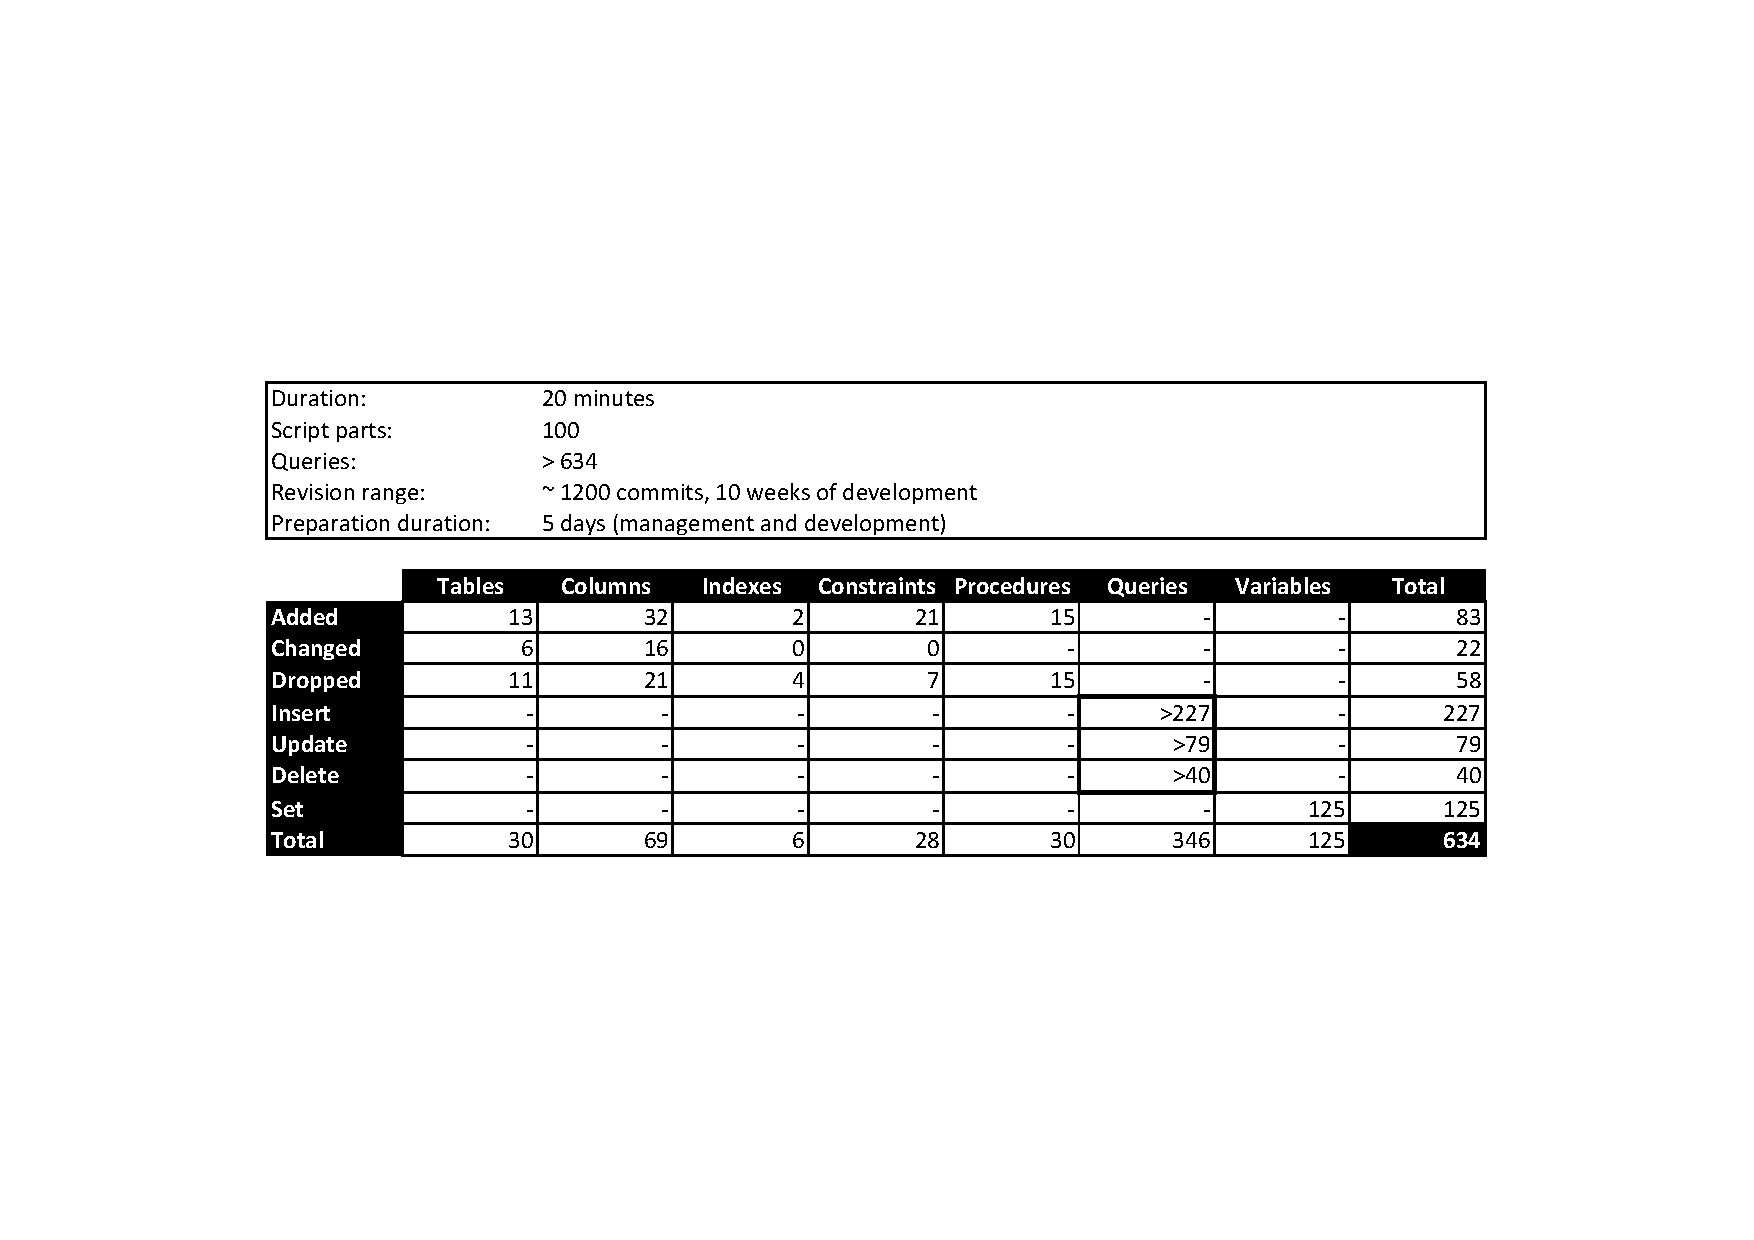
\includegraphics[scale=0.65]{images/Statistics_mig2.pdf}
        \caption{Migrations with a basic process}
        \label{fig:Statistics_mig2}
\end{figure}

Nevertheless, we had reduce the preparation time for a migration. The sample migration on \autoref{fig:Statistics_mig2} shows the growth of commits for a migration with a direct impact of the number of migration script parts. By the way, the statistics were handled in the same way than the previous migrations with count from the migration scripts to. They remain basic and not totally relevant.

\subsection{Migration with an enhanced framework}

At this stage, we had put in place improved rules that the developer team could have access and could use to write the migration script parts. The rules try to cover all the aspects we need. From the previous rules we proposed, we have done some modifications to match the technologies, tools and frameworks. For example, we replaced the numbering rules by revision number usage from the Subversion info. Each commit from repository in Subversion is tagged with a unique revision number that we can use. It allows to know that a migration script part referred to a specific revision that introduced the schema or data change. These changes show that our framework is quite flexible that could be adapted to a specific environment. Aside these changes, the rules remain the same and were used in the state we presented them.

Another improvement we did was the tool. We continued to developed the script building tool with the algorithm we presented in pseudo code \autoref{pcode:buildingScript1} and followings. We also introduced the enrichment of scripts with the queries for automatic metering. From this point, the metrics we gathered are not obtained by hand but directly from the database. As we use MySQL, we have specialized our tool. We use directly database informational schema to gather the metrics. MySQL offers some statistical data like number of queries, number of inserts, number of updates and so on. We manipulate these values to calculate our metrics that we will store directly into the application database tables.

We have also added some tables into the application database schema to keep migration information from time to time. Each migration will populate the additional tables with the metrics values, migration info and so on. We use exactly what we have explained in \autoref{sec:migInfoAndStats}. These information have multiple usage in addition to have interesting data about the data migration. We can follow each migration and from an audit point of view, these data are really useful.

Last but not the least, we have introduced all these new artifacts to the developers. We convinced each developer to follow the rules and why it is important to follow the rules. It was not an easy task due to the fact that each developer has his own habits. It is clearly important that the development team understand the goals to be strict about migration process. They have a major role to play in the process by writing atomic migration part that correspond to any data model changes. We must be able to reproduce at any time any migration from scratch.

\begin{figure}[h]
        \centering
        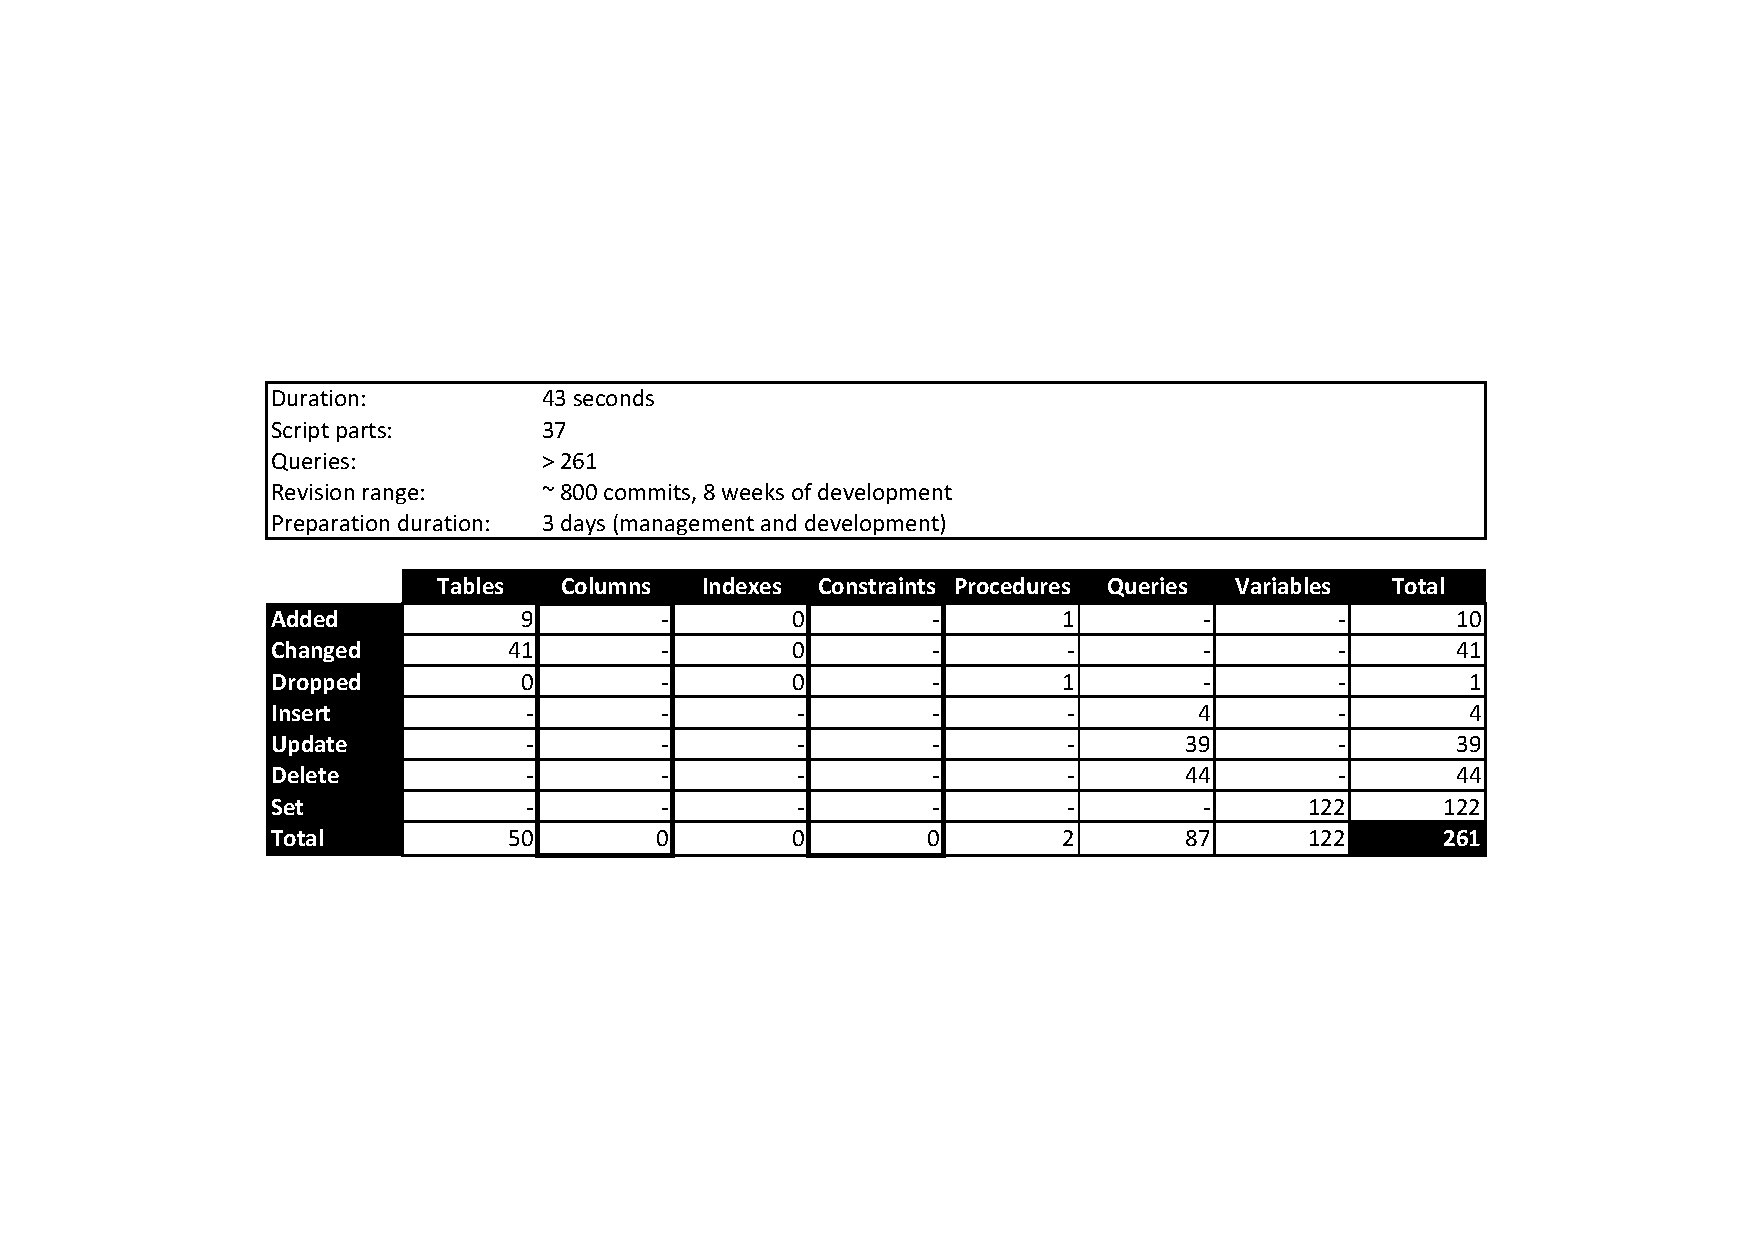
\includegraphics[scale=0.65]{images/Statistics_mig3.pdf}
        \caption{Migration with an enhanced process}
        \label{fig:Statistics_mig3}
\end{figure}

The migration statistics example in \autoref{fig:Statistics_mig3} shows that we can handle migrations with ease. The total of commits remains important but the preparation time was reduced. The time to invest in a migration starts to be reasonable. We can also see that the statistics are quite strange. There are no data for the constraints and columns but the script contains modification for these kind of modifications. We suppose that the metrics that we gather automatically from MySQL are not present directly. We have probably these data confused in other metrics like table modifications. We have to investigate and correct these errors but it is clearly an improvement than doing by hand.

\subsection{Evolution summary}

As we have described, the evolution of our methods to migrate our applications conduct us to develop tools, process and rules. Without these, we clearly loose time and improve the risks of errors. We know that we have a long road to cross to reach a more satisfying situation. We absolutely need robustness and confidence in our migration scripts that we do not have so much actually. We need to think about testing our migrations as soon as possible in the whole process to preventively detect any defect.






\section{Future work}

As we have discussed, our framework is usable in the current state but missed from some points like tests. We have also see that we can improve some aspects of our tools and rules.

\subsection{Testing framework}

To test our migration, the first step we can do is to compare a database that is populated as a new application deployment, in our case, our ORM could do this in development environment, and a database that is managed as production one. It means that the second database is populated and migrated from the migration scripts. Comparing the both database schema enforce the confidence that there is no difference between a newly deployed application from a same version than one that is migrated. The comparison required a tool that is able to compare table schema, constraints, indexes and so on. We could write our own tool or investigate for a tool on the market. It seems to be a quite common need but our preliminary researches for such a tool were not a success.

This kind of tools will not take into account the data into the database, for that we need another tool or process. Our first reflexions for that conducts us in a way that each migration script must contains queries that could be able to test the validity of the migration. Idea is to follow some kind of unit testing. It is probably sufficient for most of the migration but some of them will probably require more than simple queries. We need to think about advanced requirements to test data.

\subsection{Building tool improvements}

Actually, we do not have any simple validation of the queries that are written. A good solution is to improve the script building tool with a validation framework that enable to check the correctness of the SQL queries written. These verifications will manage syntax errors but not the semantic errors. These ones could only be handled by solution we have just described in previous section. The framework we want to add in our tool must be flexible that it could be possible to add easily new rules when new kind of errors are discovered. For example, we want to enforce that each query is prefixed by the correct database to avoid running queries agains the wrong database if erroneous database is selected at the script runtime.

A second axe that we want to improved is the data and metrics we gathered around the migration. We want to add more details for each migration parts. For example, we want to add the person who wrote the migration and the person who wrote the modification. In the majority of the cases, it will be the same but sometimes not. When this is not the case, it could be interesting to understand why there was two persons involved in the migration script part. Gathering the comments from the versioning tool is also useful to keep track of migration against code modifications. They are a lot of data that we can retrieve to enrich the migration data.

Finally, we would also improve the metrics that we calculate and analyze them. It allows to see the trends of migrations, by which script / queries the time is consumed by a migration. As we run migration in pre-production environment, these data could be used to improve the migration scripts before running them into a real environment.

\subsection{Automatic builds}

The previous improvement will logically conduct us to the automation of the building process. The concept of nightly build is relatively widespread. We want to use this concept also for the migration process. Idea is to build the migration script every night and to run it agains a database in a state to be migrate. With a comparator tool and other testing tools, we could put all together and construct an automation of building, running and testing a migration script. This allows to be pretty ready every day for a migration. Unfortunately, it is only possible to use such an approach if we have sufficient testing tools.

\subsection{Tracking}

As we have described, we want to add a validation framework to our building tool. This is clearly useful and help us to save time in debugging process but it is not sufficient. The building tool is only used when a migration is prepared and this is near the end of the whole process. It occurs too late in the migration process. One other solution is to add this validation process in the same way that we track any changes in data model in the code. We could add these validations at the commit time to ensure the scripts are basically correct and forbid the commit if the script contains errors. This way will, for sure, save a lot of time for the migration manager.

\section{conclusion}




\bibliographystyle{plain}
\bibliography{pa}
\end{document}
